\documentclass[11pt]{article}

\usepackage[preprint]{acl}

\usepackage{times}
\usepackage{latexsym}
\usepackage[T1]{fontenc}
\usepackage[utf8]{inputenc}
\usepackage{microtype}
\usepackage{xurl}
\usepackage{graphicx}
\usepackage{booktabs}
\usepackage{multirow}
\usepackage{amsmath}
\usepackage{amssymb}
\usepackage{xcolor}
\usepackage{enumitem}
\setlist{nosep,leftmargin=1.2em}

\graphicspath{{figures/}}
\emergencystretch=2em
% let LaTeX place more figures per page, closer to where they are cited
\usepackage{dblfloatfix}
\renewcommand{\topfraction}{0.9}
\renewcommand{\bottomfraction}{0.6}
\renewcommand{\textfraction}{0.07}
\renewcommand{\floatpagefraction}{0.85}
\renewcommand{\dbltopfraction}{0.9}
\renewcommand{\dblfloatpagefraction}{0.85}
\setcounter{topnumber}{3}
\setcounter{totalnumber}{5}
\setcounter{dbltopnumber}{2}
\sloppy

% short box explaining how to read a figure
\newcommand{\howtoread}[1]{\par\smallskip\noindent\fcolorbox{gray!45}{gray!6}{\parbox{\dimexpr\linewidth-2\fboxsep-2\fboxrule}{\small\textit{How to read it.} #1}}\par\smallskip}

\title{Do Events Move Online Hate? Hate Speech Toward Migrants Around\\
Social and Political Events on Polish Wykop, YouTube and Bluesky}

% TODO: affiliation and e-mail addresses
\author{Julia Sołtys \and Małgorzata Skowron \and Marta Torzyńska \and Aleksandra Walczybok \\
  Digital Media Analysis course project \\
  \texttt{\{e-mail\}}}

\begin{document}
\maketitle

\begin{abstract}
We study whether salient social and political events related to migration change the amount of hate speech toward migrants in Polish-language social media, and whether this depends on the type of event and on the platform. We collected 1.66 million comments from Wykop, YouTube and Bluesky around 15 events from 2022--2026. Comments were labelled in two independent ways: with a HerBERT hate-speech classifier (general hate, 11 events) and with a local large language model (hate toward migrants, 7 events), both combined with a dictionary of ethnic slurs and evaluated on a 600-comment gold standard. For each event and platform we compare the 7 days before and the 15 days after the event with odds ratios and combine the results with a random-effects meta-analysis. Some events clearly increase hate -- most of all the adoption of the EU Pact on Migration and Asylum -- but others decrease it, and on average there is no effect (pooled OR = 1.03 for both labelling methods). Where hate grows, it grows because more people write about migration, not because the discussion becomes more hostile. The type of event does not explain the size of the reaction, and the platforms differ in how much hate they contain rather than in how they react. Finally, we describe what hateful comments look like: they are marked by profanity, dehumanising words and ideological labels rather than by mentions of a particular group, and they are written by many occasional users rather than by a few dedicated accounts.
\end{abstract}

\noindent\textbf{Keywords:} hate speech, migration, social media, Polish, event study, meta-analysis, LLM classification

% =====================================================================
\section{Introduction}

Migration has been one of the most divisive topics in Polish public debate for the last decade. After the full-scale Russian invasion of Ukraine in 2022, Poland received a large number of refugees from Ukraine; at the same time the crisis on the Polish--Belarusian border and the EU Pact on Migration and Asylum kept migration high on the political agenda. Much of this debate takes place online, and hostile content is common there: in 2025, 42.3\% of internet users in the EU reported seeing hostile or degrading messages online, and 25.5\% saw such messages targeting racial or ethnic origin \citep{eurostat2026}. In Poland, a study of Polish Twitter found that the most popular posts about Ukrainians often presented them as taking over Polish culture, carried negative sentiment and frequently spread disinformation \citep{lipinska2025}.

The level of online hate is not constant. Research from other countries shows that hateful messages can increase sharply after trigger events such as terrorist attacks \citep{williams2016,olteanu2018}, and that online hostility toward minorities is linked to offline hate crime \citep{muller2021}. It is less clear whether this pattern is general: do different kinds of events -- political decisions, crimes, disinformation, border crises -- move hate in the same way, and do different platforms react in the same way?

In this paper we study hate speech toward migrants in Polish-language comments on three platforms with different users and moderation rules: Wykop, YouTube and Bluesky. We collect comments around 15 major events from 2022--2026 that were widely covered in Polish media. We label them with two independent methods -- a transformer classifier and a local large language model (LLM) -- and evaluate both on a gold standard in which every disagreement between annotators was resolved by a person. We then test three hypotheses:

\begin{itemize}
  \item \textbf{H1 (event effect):} after a major event related to migration, the level of hate speech toward migrants changes;
  \item \textbf{H2 (event type):} the strength and direction of the change depend on the type of event (criminal, political, disinformation, border crisis);
  \item \textbf{H3 (platforms):} the relationship between events and hate speech differs between Wykop, YouTube and Bluesky.
\end{itemize}

\noindent Beyond the hypotheses, we ask two additional questions: \textbf{(Q1)} what hate toward migrants is about -- which words it uses, whom it targets and who writes it, and \textbf{(Q2)} how hateful comments differ from other comments in discussions about migration -- in their language, length, the reactions they receive and their authors.

Our contributions are:
\begin{enumerate}
  \item \textbf{An end-to-end, reusable pipeline.} The user only specifies the platform and the event dates; the pipeline then collects the posts and comments in a time window around each event, cleans and pseudonymises them, filters comments related to migration, labels them with both methods and runs the statistical analyses that produce the final tables and figures.
  \item \textbf{A comparison of reactions to 15 events on three Polish platforms.}
  \item \textbf{Two independent labelling methods evaluated on the same gold standard.} Every result is computed twice, with the classifier and with the LLM, so we can check that a finding does not depend on one particular model.
  \item \textbf{An analysis framework based on odds ratios and meta-analysis}, which makes it possible to compare events and platforms with very different amounts of data.
\end{enumerate}

% =====================================================================
\section{Related Work}

\paragraph{Hate speech toward migrants and events.} Hate speech toward migrants is a well-studied topic; the SemEval-2019 HatEval task, for example, focused specifically on hate toward immigrants and women on Twitter \citep{basile2019}. Several studies have examined how online hate reacts to events. \citet{williams2016} analysed how anti-Muslim hate on Twitter escalated, spread and then de-escalated after a soldier was murdered in a terrorist attack in Woolwich, London. \citet{olteanu2018} found that after Islamist terrorist attacks, hateful speech against Muslims and Arabs increased on both Twitter and Reddit over the following week -- especially messages that call for violence -- and that the effects differed between the two platforms. In the Polish context, \citet{lipinska2025} analysed anti-Ukrainian narratives on Polish Twitter, and \citet{linkeviciute2025} studied hate speech toward war refugees from Ukraine in Lithuanian news comments. Most of these studies examine a single event or a single platform; we compare many events and three platforms with the same method.

\paragraph{Automatic hate speech detection.} Early approaches used classical machine learning on word and n-gram features. \citet{davidson2017} showed that such models easily confuse hate speech with language that is merely offensive, which leads to many false positives \citep[see also the survey by][]{fortuna2018}. A recent review of more than 100 studies \citep{ramos2024} concludes that transformer models such as BERT and RoBERTa now give the best results, but require much more computing power than earlier methods. The main remaining problems are bias in the models, the small amount of labelled data, especially for languages other than English, and the fact that hate-speech systems are usually tested on different datasets, which makes them hard to compare.

\paragraph{Polish models and data.} For Polish, the PolEval 2019 shared task introduced the first dataset for cyberbullying detection on Twitter \citep{ptaszynski2019}. This dataset later became the CBD task of KLEJ, the standard benchmark for Polish language understanding \citep{rybak2020klej}. Results on CBD show how quickly the field has progressed. The first Polish BERT models reached an F1 of about 50 \citep{rybak2020klej}. Polish RoBERTa-large reached 71.1 and multilingual XLM-R large 70.6 \citep{dadas2020}. TrelBERT, a model pre-trained on Polish tweets, reached 76.1 \citep{szmyd2023trelbert}. BAN-PL \citep{kolos2024banpl} is a large dataset of content removed by the moderators of Wykop, one of our platforms. The publicly available hate-speech classifier that we use is based on the Polish model HerBERT \citep{mroczkowski2021,kleczek_herbert_hs}. More recently, large language models (LLMs) have been used as annotators, reaching accuracy comparable to that of crowd workers \citep{gilardi2023}. They can take the context of a comment into account, but their results depend on the prompt and they are costly to run at scale.

% =====================================================================
\section{Data Sources}

\paragraph{Wykop} (\url{https://wykop.pl}) is a Polish social news aggregator, similar to Reddit: users post links and short entries, and others comment and vote them up or down. It is one of the largest Polish-language discussion platforms. We used the official Wykop API.

\paragraph{YouTube} is the most widely used social media platform in Poland. Polish news and political channels publish videos about current events, and their comment sections are very active. We used the YouTube Data API v3.

\paragraph{Bluesky} (\url{https://bsky.app}) is a decentralised microblogging platform that grew quickly in 2024--2025 as users left X/Twitter \citep{seckin2025bluesky}. Its Polish-language community is small, especially before 2024, which limits the analysis of older events. We used the open AT Protocol API.

% =====================================================================
\section{Data Collection}

\paragraph{Events.} We selected 15 events from 2022--2026 that were widely covered in Polish media and related to migration (Table~\ref{tab:events}). Each event was assigned one type: \emph{criminal}, \emph{political}, \emph{disinformation}, \emph{border crisis} or \emph{war}.

\begin{table}[tbp]
\centering
\small
\setlength{\tabcolsep}{3pt}
\begin{tabular}{@{}lllcc@{}}
\toprule
Date & Event & Type & H & L \\
\midrule
2022-02-24 & Russian invasion of Ukraine & war & & \\
2022-05-08 & Murder in Warsaw & disinformation & & \\
2023-09-22 & Film \textit{Green Border} & political & & \\
2023-10-15 & Election and referendum & political & & \\
2024-04-10 & EU Pact adopted & political & \checkmark & \checkmark \\
2024-05-28 & Attack on a soldier & criminal & \checkmark & \\
2024-06-06 & Death of the soldier & criminal & \checkmark & \checkmark \\
2024-09-08 & Brawl in Śrem & criminal & \checkmark & \checkmark \\
2024-10-12 & Migration strategy & political & \checkmark & \checkmark \\
2025-06-06 & ICE raids, LA & political & \checkmark & \\
2025-10-15 & Kraków murder & disinformation & \checkmark & \checkmark \\
2026-06-12 & EU Pact in force & political & \checkmark & \\
2026-07-30 & Ceuta mass crossing & border crisis & \checkmark & \checkmark \\
2026-08-15 & Kamienna Góra attack & criminal & \checkmark & \checkmark \\
2026-09-15 & Jarosław attack & criminal & \checkmark & \\
\bottomrule
\end{tabular}
\caption{Events. ``Murder in Warsaw'' and ``Kraków murder'' were cases of disinformation about the perpetrator. H: included in the HerBERT analysis (11 events); L: included in the LLM analysis (7 events). The first four events were collected only on YouTube.}
\label{tab:events}
\end{table}

\paragraph{Collection.} On \textbf{Wykop} and \textbf{Bluesky} we searched for posts with a dictionary of migration-related keywords and downloaded all comments under the posts found, from 28 days before to 28 days after the event. On \textbf{YouTube}, API limits made a platform-wide keyword search too costly. Instead, we downloaded all top-level comments under videos published by ten Polish news and political channels (TVN24, Kanał Zero, ORB, Onet, Telewizja Republika, polsatnews.pl, TVP Info, Razem, Sławomir Mentzen, Praktycznie o pieniądzach), from 7 days before to 14 days after the event. This gives many more comments, but many of them are not about migration.

In total we collected \textbf{1.66 million comments}: 255,857 from Wykop, 1,228,811 from YouTube and 175,103 from Bluesky. For each comment we kept its text, date, thread, the comment it replies to and the number of likes and replies.

\paragraph{Pseudonymisation.} User names and identifiers were replaced with random codes, and mentions of other users were removed from the text. The data are used for research only and are not published.

% =====================================================================
\section{Preprocessing and Filtering}

\paragraph{Cleaning.} We removed links, user mentions, emoji and quotations of other comments, so that each text contains only the words of its author. This cleaned text is the input to all classifiers. The original text, with emoji and capital letters, was kept and is used only in Q2 (Section~\ref{sec:q2}), where we count emoji and capital letters.

\paragraph{Topic filter.} A comment was kept as potentially related to migration if the comment or the post it belongs to contained a word from the migration keyword dictionary (e.g.\ \textit{migrant}, \textit{uchodźca} `refugee', \textit{Ukrainiec} `Ukrainian') or an ethnic slur. The filter kept 452,455 comments. The share of comments that passed the filter differs strongly between platforms, because of the different collection methods: 72--83\% on Wykop, 5--44\% on YouTube and 10--36\% on Bluesky, depending on the event. For this reason we compare the \emph{level} of hate only within a platform, and between platforms we compare only \emph{changes}.

\paragraph{Analysis window.} All analyses use the same window: 7 days before the event (days $-7$ to $-1$) and 15 days after it (days $0$ to $+14$). The unit of observation is a single comment, which is labelled as hateful or not. Effects, however, are estimated for groups of comments: we call one event on one platform a \emph{cell} (e.g.\ the EU Pact on Wykop) and, within each cell, compare comments posted before the event with comments posted after it. Cells with fewer than 30 comments before or after the event are not used to estimate effects. The YouTube cell for the soldier's death was excluded, because all of its pre-event comments come from a single video.

% =====================================================================
\section{Classification}

\subsection{Labels}
We use three binary labels:
\begin{itemize}
  \item \texttt{migrant}: the comment is about migrants or migration;
  \item \texttt{hate}: the comment attacks anyone -- with insults, dehumanisation, stereotypes, calls for exclusion or violence;
  \item \texttt{hate\_migrant}: the attack targets migrants (including Ukrainians) because of their origin or status.
\end{itemize}
Hate toward politicians, other users, ``leftists'' or Russians is \texttt{hate} but not \texttt{hate\_migrant}. Criticism of a law or of a state, without attacking people, is neither. The rules, with examples, are written down in a codebook.

\subsection{Two labelling pipelines}

Both pipelines start with a \textbf{dictionary of ethnic slurs}: a comment containing an unambiguous slur against migrants is labelled $\texttt{hate} = \texttt{hate\_migrant} = 1$ (Figure~\ref{fig:pipeline}).

\paragraph{Classifiers (label \texttt{hate}).} Comments that pass the topic filter are classified by three Polish transformer models: (1) HerBERT-large fine-tuned for hate-speech detection \citep{kleczek_herbert_hs,mroczkowski2021}; (2) Polish BERT fine-tuned for cyberbullying detection on PolEval data \citep{ptaszynski2019}; (3) Polish RoBERTa that we fine-tuned on BAN-PL \citep{kolos2024banpl}. A comment is hateful if the predicted probability is at least 0.5. HerBERT was the best model on the gold standard (Section~\ref{sec:gold}) and is used in all further analyses.

\paragraph{LLM (labels \texttt{migrant}, \texttt{hate}, \texttt{hate\_migrant}).} We used Qwen2.5 with 7B parameters \citep{qwen2024}, run locally with Ollama, so that the data never left our computers. The model sees the comment together with the post and the comment it replies to. It first decides whether the comment is about migration; only comments about migration receive the \texttt{hate} and \texttt{hate\_migrant} labels. Running the model locally was slow, so prompts had to be short and the context limited.

\begin{figure*}[t]
  \centering
  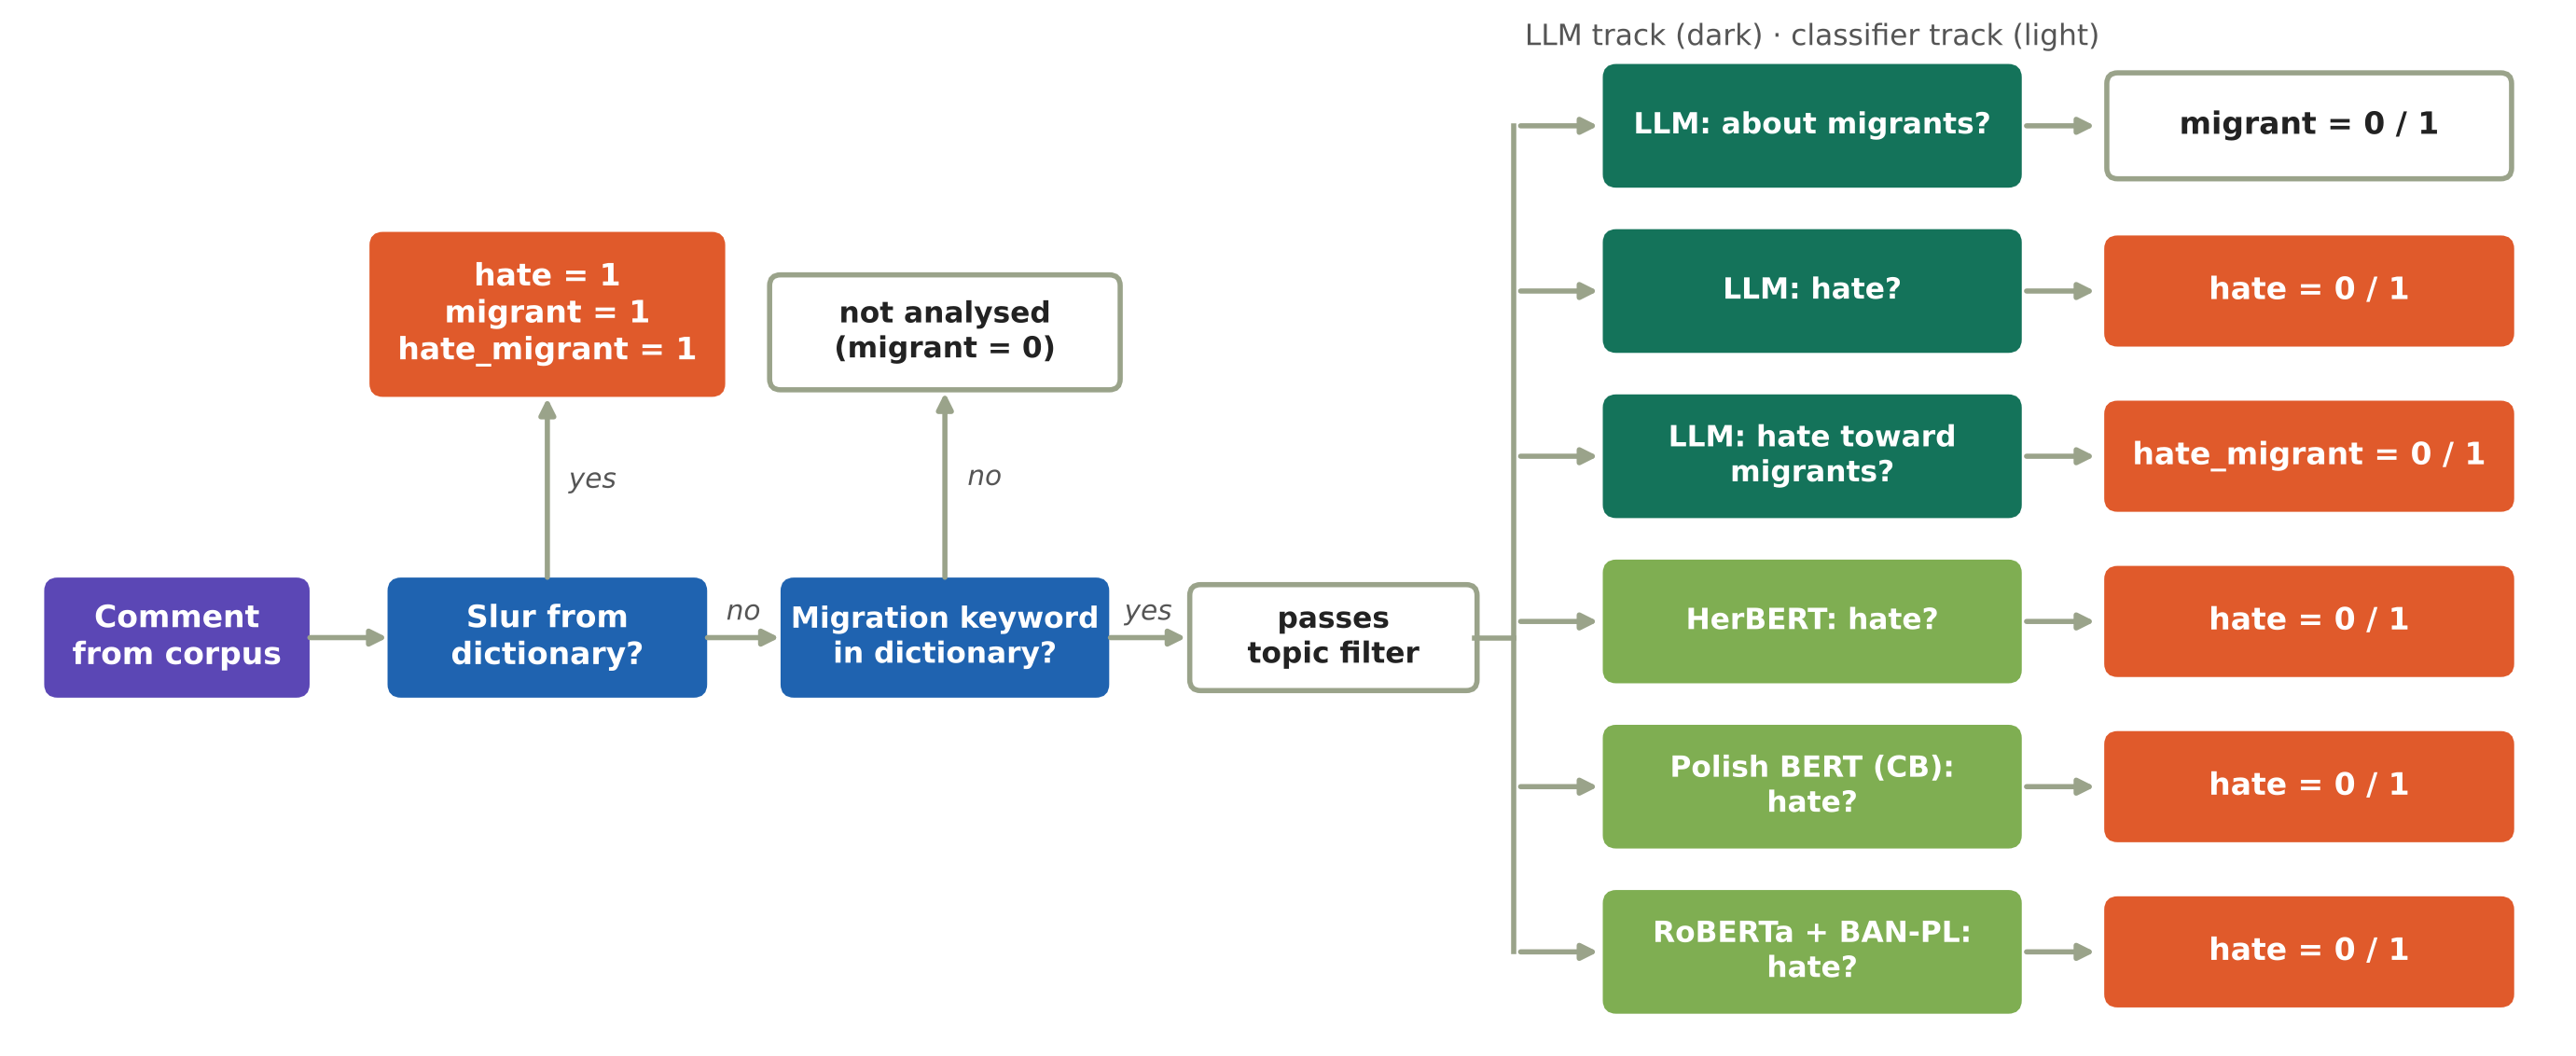
\includegraphics[width=0.9\textwidth]{fig_pipeline_en.png}
  \caption{Labelling pipeline. A comment with a slur from the dictionary is labelled as hate toward migrants directly. Otherwise, comments that contain a migration keyword pass the topic filter and are labelled by the LLM (dark green: is it about migrants? is it hate? is it hate toward migrants?) and by three classifiers (light green: is it hate?). Comments without a migration keyword are not analysed.}
  \label{fig:pipeline}
\end{figure*}

\subsection{Gold standard}
\label{sec:gold}

\paragraph{Pilot rounds: people and LLMs.} We first developed the codebook in two pilot rounds of 100 comments each (one from Bluesky, one from Wykop). In both rounds, all four authors labelled the same comments independently. People often disagreed: Krippendorff's $\alpha$ \citep{krippendorff2004} was 0.40 and 0.43 for \texttt{hate} and 0.32 and 0.34 for \texttt{hate\_migrant}, which shows how ambiguous short online comments are. After each round we discussed the disagreements and made the codebook more precise.

In the second round, two LLM annotators (Claude and Gemini) labelled the same 100 comments, using the full codebook as instructions. We then checked how often each annotator agreed with the majority decision of the people. For the LLMs this was 74--78\% of comments for \texttt{hate} and 84--85\% for \texttt{hate\_migrant}; for each of the four authors, compared with the other three, it was 71--82\% and 75--86\%. In other words, the LLMs agreed with the human majority as often as the people agreed with each other, so we used them to label the larger gold standard, with every disagreement resolved by a person.

\paragraph{Final gold standard.} The gold standard contains \textbf{600 comments}, 200 per platform, from the 7 events of the LLM analysis. To include enough difficult cases, 40\% of the comments mention migrants and contain a hostile word, 40\% mention migrants without such a word, and 20\% are hostile comments with an unclear target, posted under migration-related posts. The two LLM annotators labelled all 600 comments independently. They agreed on 83\% of comments for \texttt{hate} ($\alpha = 0.67$ [95\% CI 0.60, 0.73]) and on 90\% for \texttt{hate\_migrant} ($\alpha = 0.72$ [0.66, 0.79]). \textbf{All 113 comments on which they disagreed were resolved by a person} according to the codebook. In addition, a person checked a random 10\% of the comments on which both annotators agreed (46 comments); none had to be changed.

\subsection{Results on the gold standard}

Table~\ref{tab:gold} and Figure~\ref{fig:gold} summarise the results. For \texttt{hate}, HerBERT combined with the slur dictionary is clearly the best method (F1 = 0.78). All methods are precise (precision 0.78--0.88) but differ in how many hateful comments they find: HerBERT finds 78\%, while the other models find only 39--53\%. The LLM finds 51\% of hateful comments for \texttt{hate} and 46\% for \texttt{hate\_migrant}. The slur dictionary alone finds only a small part of hate (F1 = 0.26). All methods work worst on Bluesky, where hate is less frequent.

Because the LLM misses about half of hateful comments, it underestimates the \emph{level} of hate toward migrants. Our main analyses therefore look at \emph{changes} within the same event and platform, which are not affected by a constant miss rate, and we check every result with both pipelines.

\begin{table}[t]
\centering
\small
\setlength{\tabcolsep}{3pt}
\begin{tabular}{@{}llccc@{}}
\toprule
Label & Method & P & R & F1 \\
\midrule
\multirow{5}{*}{hate} & HerBERT + dictionary & 0.78 & 0.78 & \textbf{0.78} \\
 & Polish BERT (cyberbull.) + dict. & 0.82 & 0.53 & 0.64 \\
 & LLM + dictionary & 0.81 & 0.51 & 0.62 \\
 & RoBERTa (BAN-PL) + dict. & 0.86 & 0.39 & 0.54 \\
 & dictionary only & 0.88 & 0.15 & 0.26 \\
\midrule
hate\_migr. & LLM + dictionary & 0.61 & 0.46 & 0.53 \\
\bottomrule
\end{tabular}
\caption{Results on the 600-comment gold standard (P: precision, R: recall). In every method, comments with a slur from the dictionary are labelled as hateful before the model is applied.}
\label{tab:gold}
\end{table}

\begin{figure*}[t]
  \centering
  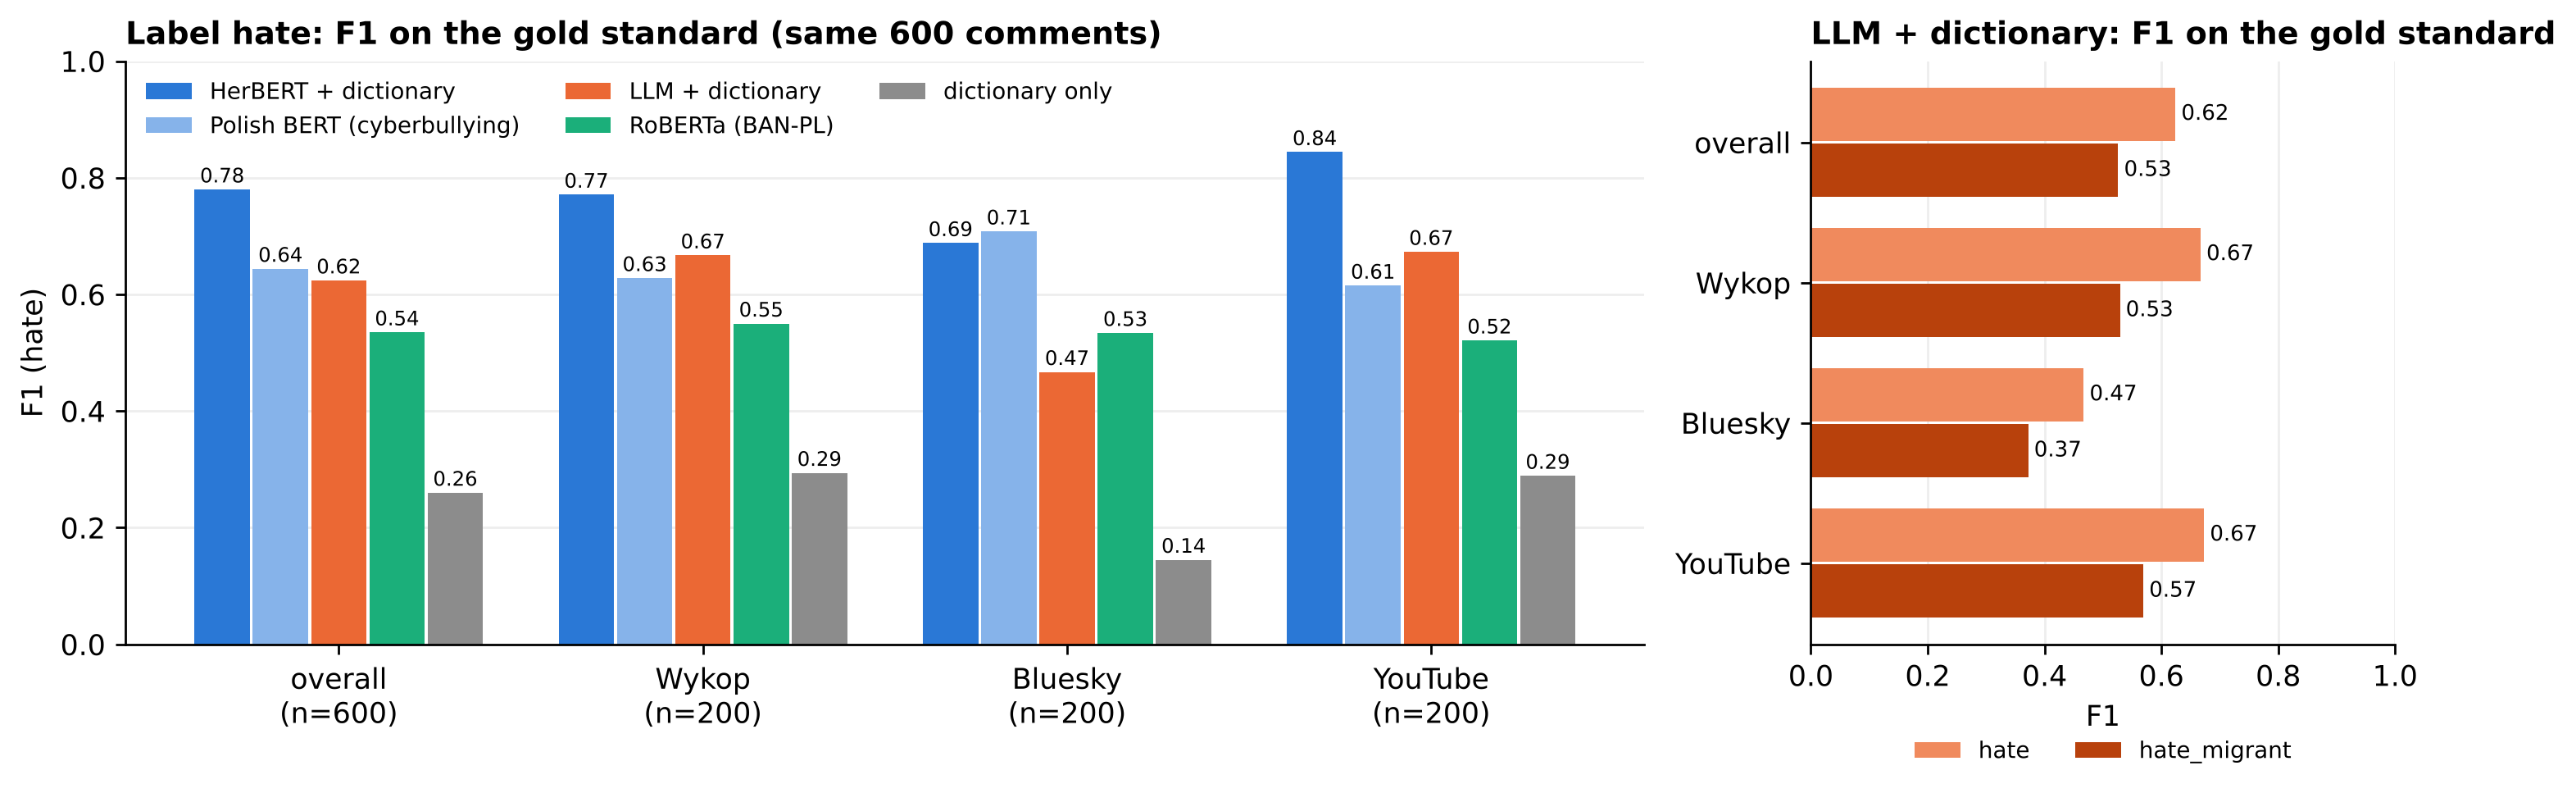
\includegraphics[width=0.9\textwidth]{fig_gold_en.png}
  \caption{F1 on the gold standard, overall ($n=600$) and per platform ($n=200$ each). Left: label \texttt{hate} for the four methods and for the slur dictionary alone. Right: the LLM with the dictionary for \texttt{hate} and \texttt{hate\_migrant}.}
  \label{fig:gold}
\end{figure*}

% =====================================================================
\section{Analysis Methods}

\paragraph{Measures.} For each cell we measure the share of hateful comments among all comments of the cell: \texttt{hate} from HerBERT (11 events) and \texttt{hate\_migrant} from the LLM (7 events). We also measure the share of comments about migration among all comments of the cell (\texttt{migrant}); a comment that did not pass the topic filter or that the LLM judged unrelated to migration counts as not about migration. This share measures how much attention migration receives, and we use it to separate attention from tone (H1).

\paragraph{Effect in one cell: the odds ratio.} Whether a comment is hateful is a yes/no outcome. The \emph{odds} of hate are the share of hateful comments divided by the share of non-hateful ones. The \textbf{odds ratio (OR)} divides the odds after the event by the odds before it. OR = 1 means no change, OR = 2 means the odds doubled, OR = 0.5 means they halved. For example, on Wykop the share of hate after the adoption of the EU Pact rose from 15.5\% to 26.2\%; the odds rose from 0.18 to 0.36, so OR = 1.94. We estimate the OR with a logistic regression and compute its confidence interval with standard errors clustered by thread, because comments in one thread are not independent. We use the OR because: (1) it follows directly from a model that takes threads into account; (2) it measures a \emph{relative} change, so platforms with very different levels of hate can be compared; (3) the logarithm of the OR is symmetric (2 and 0.5 are equally far from 1), which allows effects to be averaged. Because we test many cells, $p$-values are corrected with the Holm method \citep{holm1979}.

\paragraph{H1.} To combine all cells, we use a \textbf{random-effects meta-analysis} of the log ORs (DerSimonian--Laird with the Hartung--Knapp correction; \citealp{dersimonian1986,hartung2001}). It assumes that each event has its own true effect and estimates their average. $I^2$ measures how much of the variation between cells reflects real differences rather than chance \citep{higgins2002}. As a check, we also fit one logistic regression on all comments with a separate baseline for each cell. To see \emph{why} hate changes, we split the change into two parts: \textbf{attention} -- how many comments are about migration -- and \textbf{tone} -- how many comments about migration are hateful. Approximately, OR(hate) $\approx$ OR(attention) $\times$ OR(tone).

\paragraph{H2.} A \textbf{meta-regression} of the cell ORs on event type, controlling for platform; the $F$ test checks whether types differ. Because some types have only one event, we add a \textbf{permutation test}: we randomly reassign event types many times and count how often a random assignment gives differences at least as large as the real one.

\paragraph{H3.} The \textbf{$Q$ test} checks whether the average ORs of the three platforms differ more than their uncertainty allows. We repeat it on a \textbf{balanced panel} of events observed on all platforms, so that platforms are compared on the same events. In addition, a \textbf{Wald test} checks the interaction between the post-event period and the platform in the comment-level model.

\paragraph{Additional questions.} For Q1 we use the comments labelled \texttt{hate\_migrant}: frequent and distinctive words (weighted log-odds with a Dirichlet prior; \citealp{monroe2008}), target groups found with keyword lists, concentration of authors and likes.

For Q2 we use all comments that passed the topic filter and were labelled by HerBERT, and compare hateful with non-hateful comments. Both groups went through the same filter, so the comparison is fair, but the results describe hate in discussions about migration, not online hate in general. We describe each comment with simple, transparent keyword rules -- profanity, insults, dehumanising words, calls for exclusion, violence, exclamation and question marks, capital letters, emoji, length, addressing the reader (``you''), ``we'' and ``they'', and mentions of groups -- and fit one logistic regression of hate on all features together. The regression compares comments only within the same event and platform, so that a feature does not look important just because it is more common on a platform with more hate. Comments with a slur from the dictionary are excluded from the regression: they are labelled as hateful automatically, and since most slurs refer to Ukrainians, including them would make any mention of Ukrainians look like a sign of hate.

% =====================================================================
\section{Results}

\subsection{H1: Do events change hate?}

\begin{figure}[tbp]
  \centering
  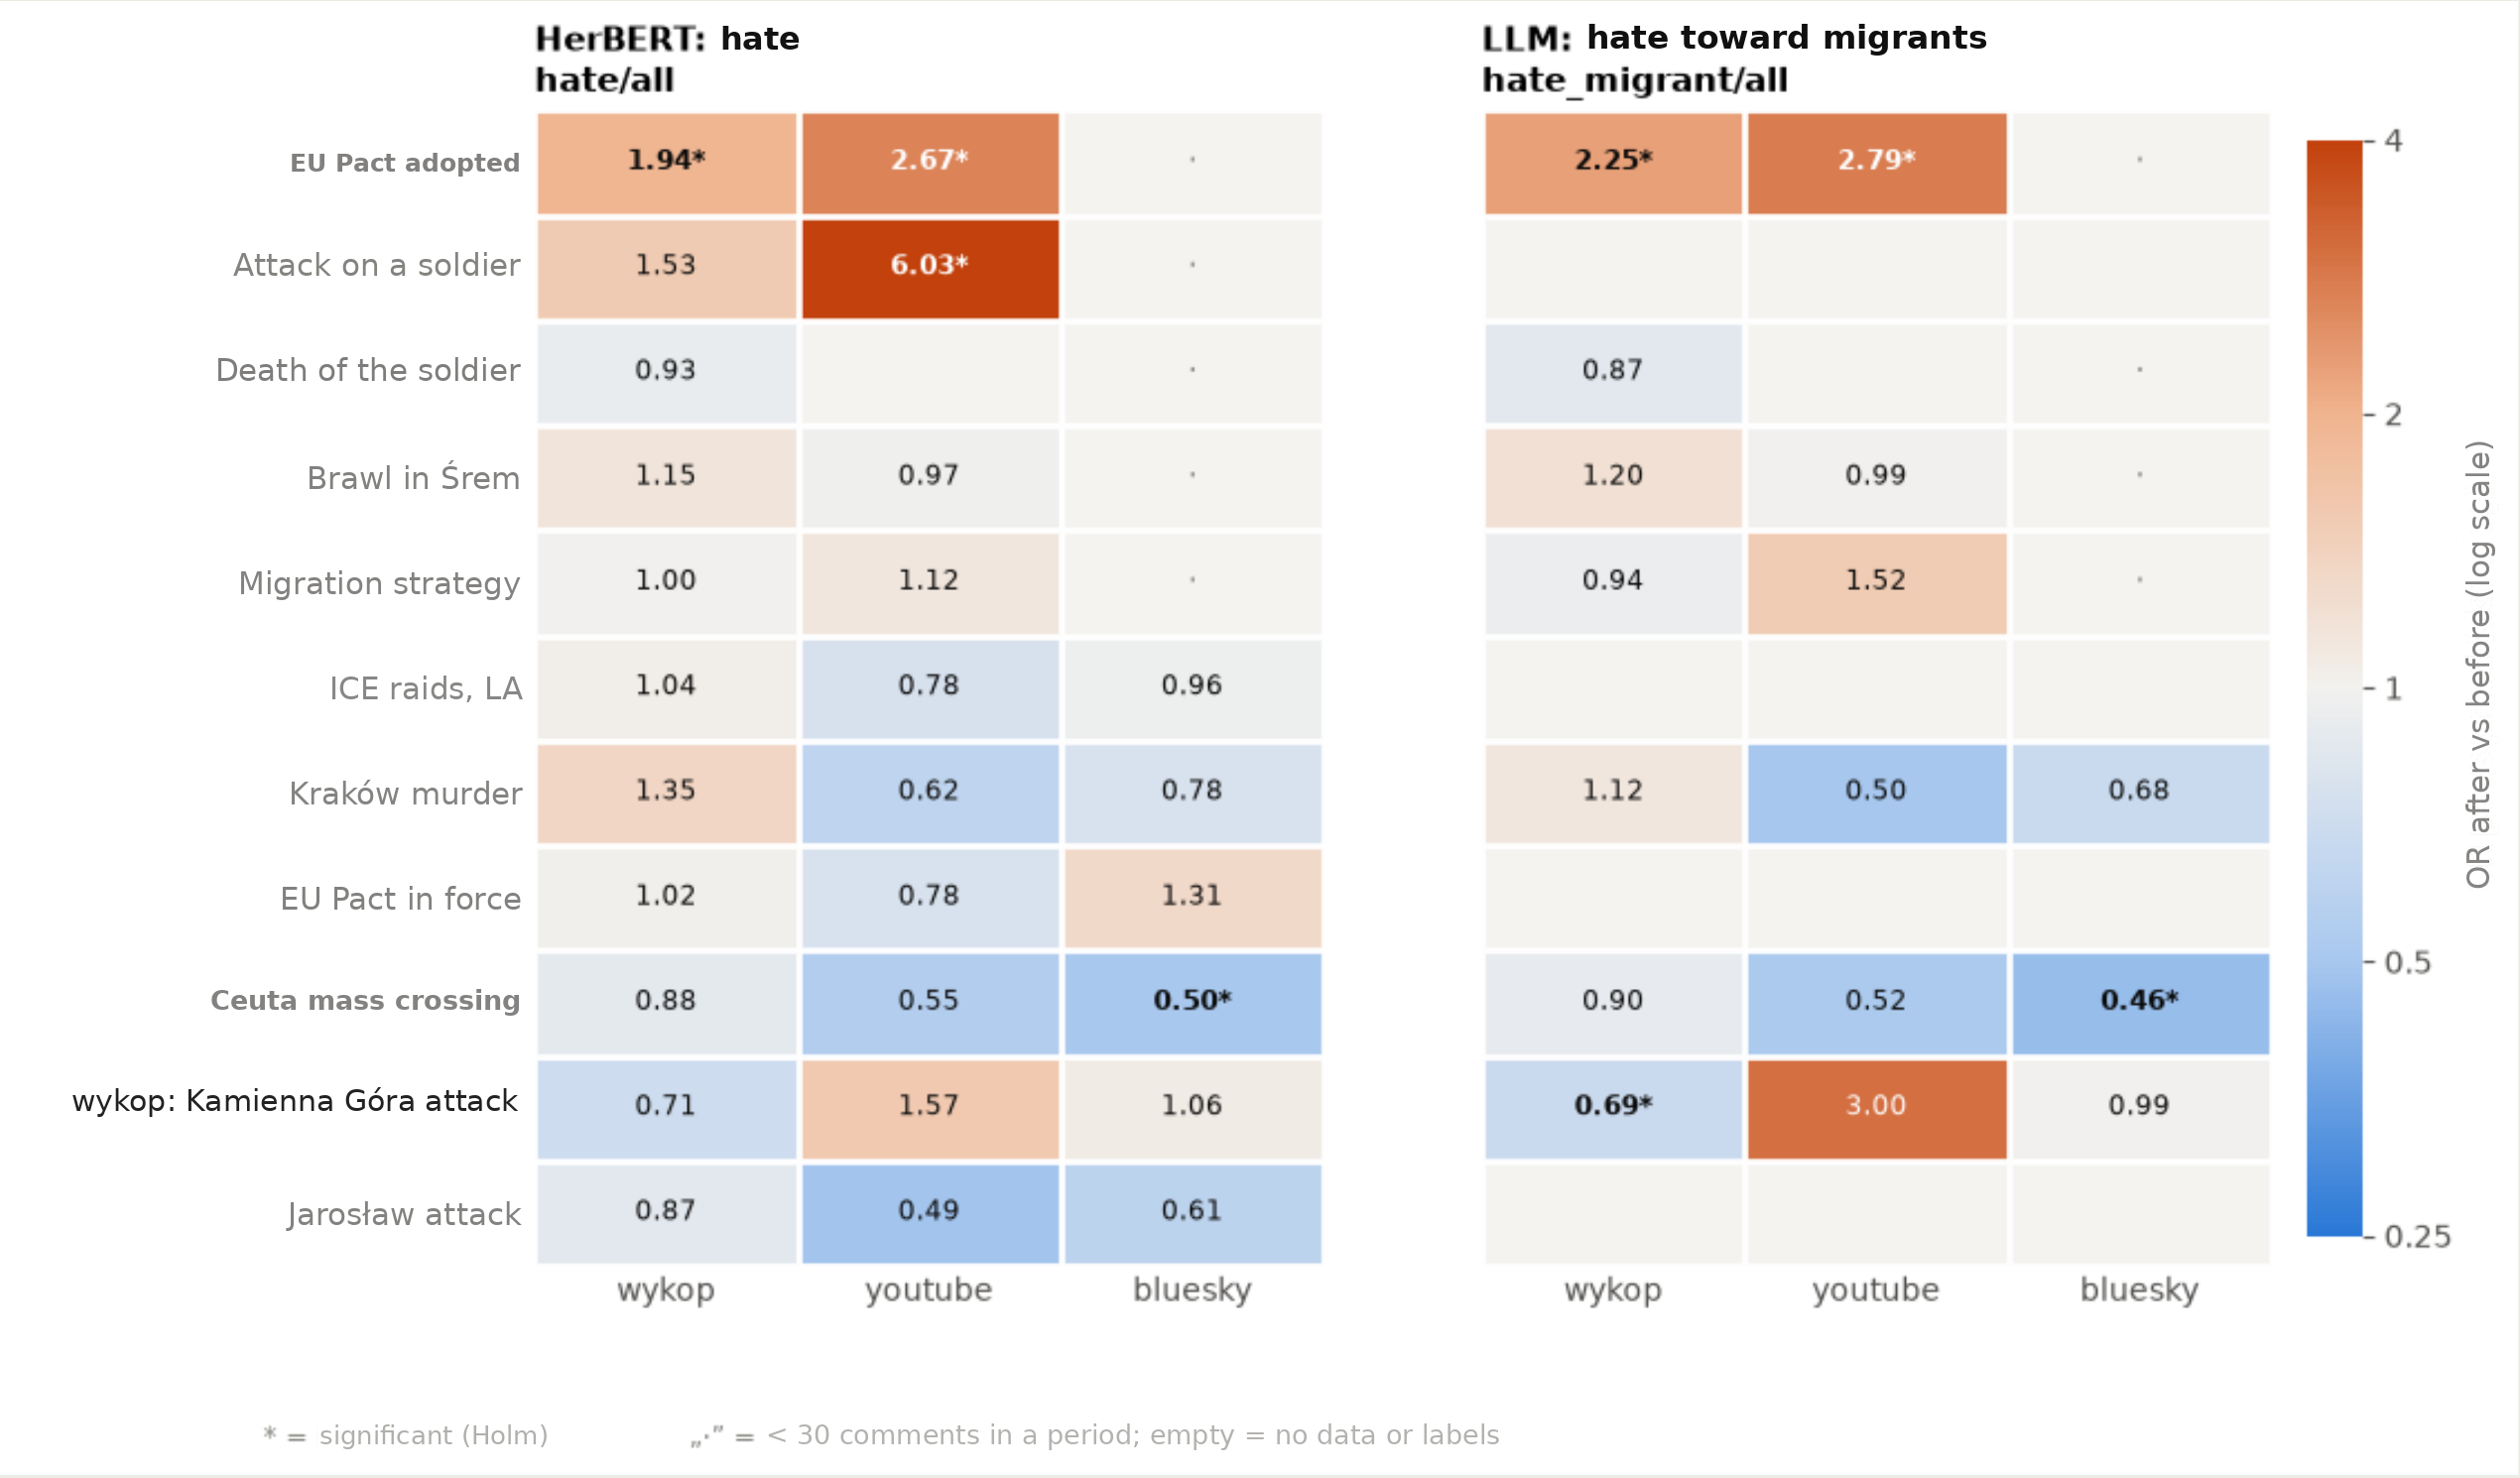
\includegraphics[width=\columnwidth]{fig_heatmap_en.png}
  \caption{OR (after vs.\ before) for each event and platform. Left: general hate (HerBERT). Right: hate toward migrants (LLM). * significant after Holm correction; ``$\cdot$'': fewer than 30 comments in a period; empty: no data.}
  \label{fig:heatmap}
\end{figure}

\howtoread{Each square in Figure~\ref{fig:heatmap} is one event on one platform. Red: more hate after the event (OR $>$ 1); blue: less (OR $<$ 1). Only squares marked with * are statistically significant.}

Most cells do not change significantly (23 of 27 HerBERT cells). Four cells change significantly in each pipeline (Figure~\ref{fig:heatmap}). The adoption of the \textbf{EU Pact on Migration and Asylum} increased hate on Wykop (OR 1.94 HerBERT; 2.25 LLM) and on YouTube (2.67; 2.79). The \textbf{attack on a soldier} on the Belarusian border increased general hate on YouTube (6.03). Hate decreased on Bluesky after the mass crossing in \textbf{Ceuta} (0.50; 0.46) and, for hate toward migrants, on Wykop after the attack in \textbf{Kamienna Góra} (0.69).

\begin{figure}[tbp]
  \centering
  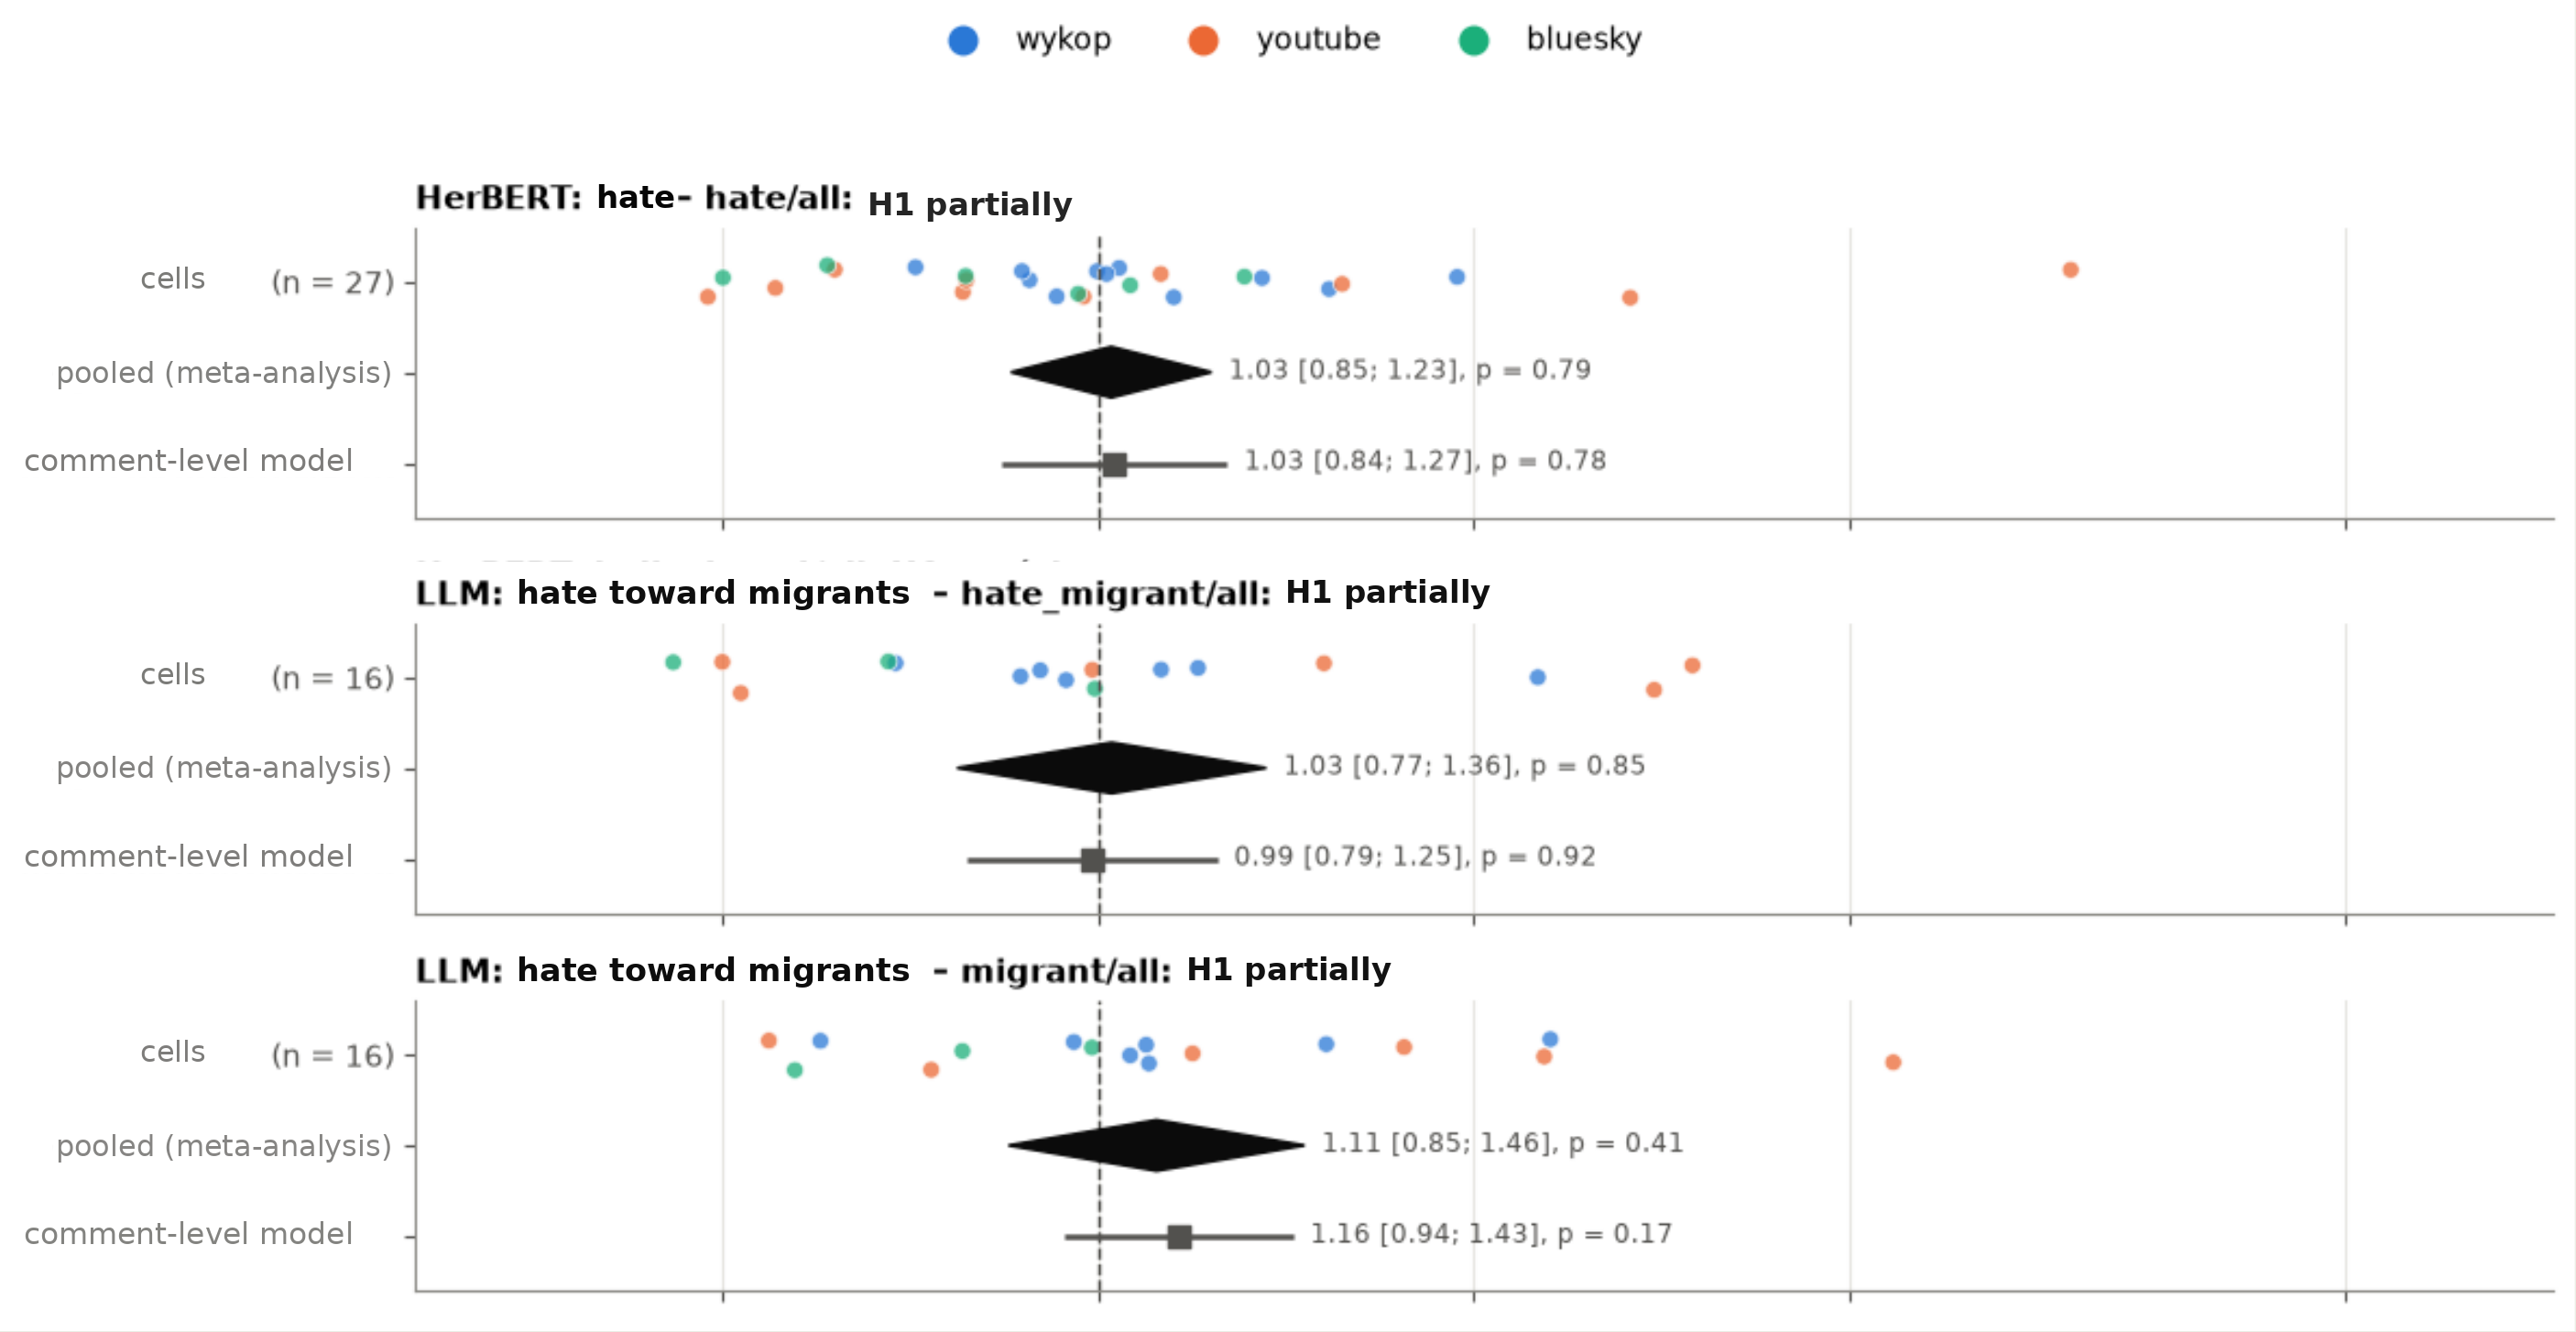
\includegraphics[width=\columnwidth]{fig_pooled_en.png}
  \caption{All cells together. Dots: individual cells (blue Wykop, orange YouTube, green Bluesky). Diamond: random-effects meta-analysis (centre = average OR, width = 95\% CI). Square: comment-level model. Panels: HerBERT \texttt{hate}; LLM \texttt{hate\_migrant}; LLM share of comments about migration (note: the third panel shows the share of comments about migration, not hate).}
  \label{fig:pooled}
\end{figure}

\howtoread{In Figure~\ref{fig:pooled}, the dashed line is OR = 1 (no change). A diamond that crosses this line means there is no significant average effect.}

On average, however, there is no effect (Figure~\ref{fig:pooled}): OR = 1.03 [0.85, 1.23], $p = 0.79$ for HerBERT and OR = 1.03 [0.77, 1.36], $p = 0.85$ for the LLM. The comment-level models give the same result (1.03, $p = 0.78$; 0.99, $p = 0.92$). Differences between cells are large ($I^2 \approx 79\%$): increases and decreases cancel each other out. We therefore cannot say that ``events increase hate'', only that \emph{some events on some platforms} do. \textbf{H1 is partially supported.}

\begin{figure*}[t]
  \centering
  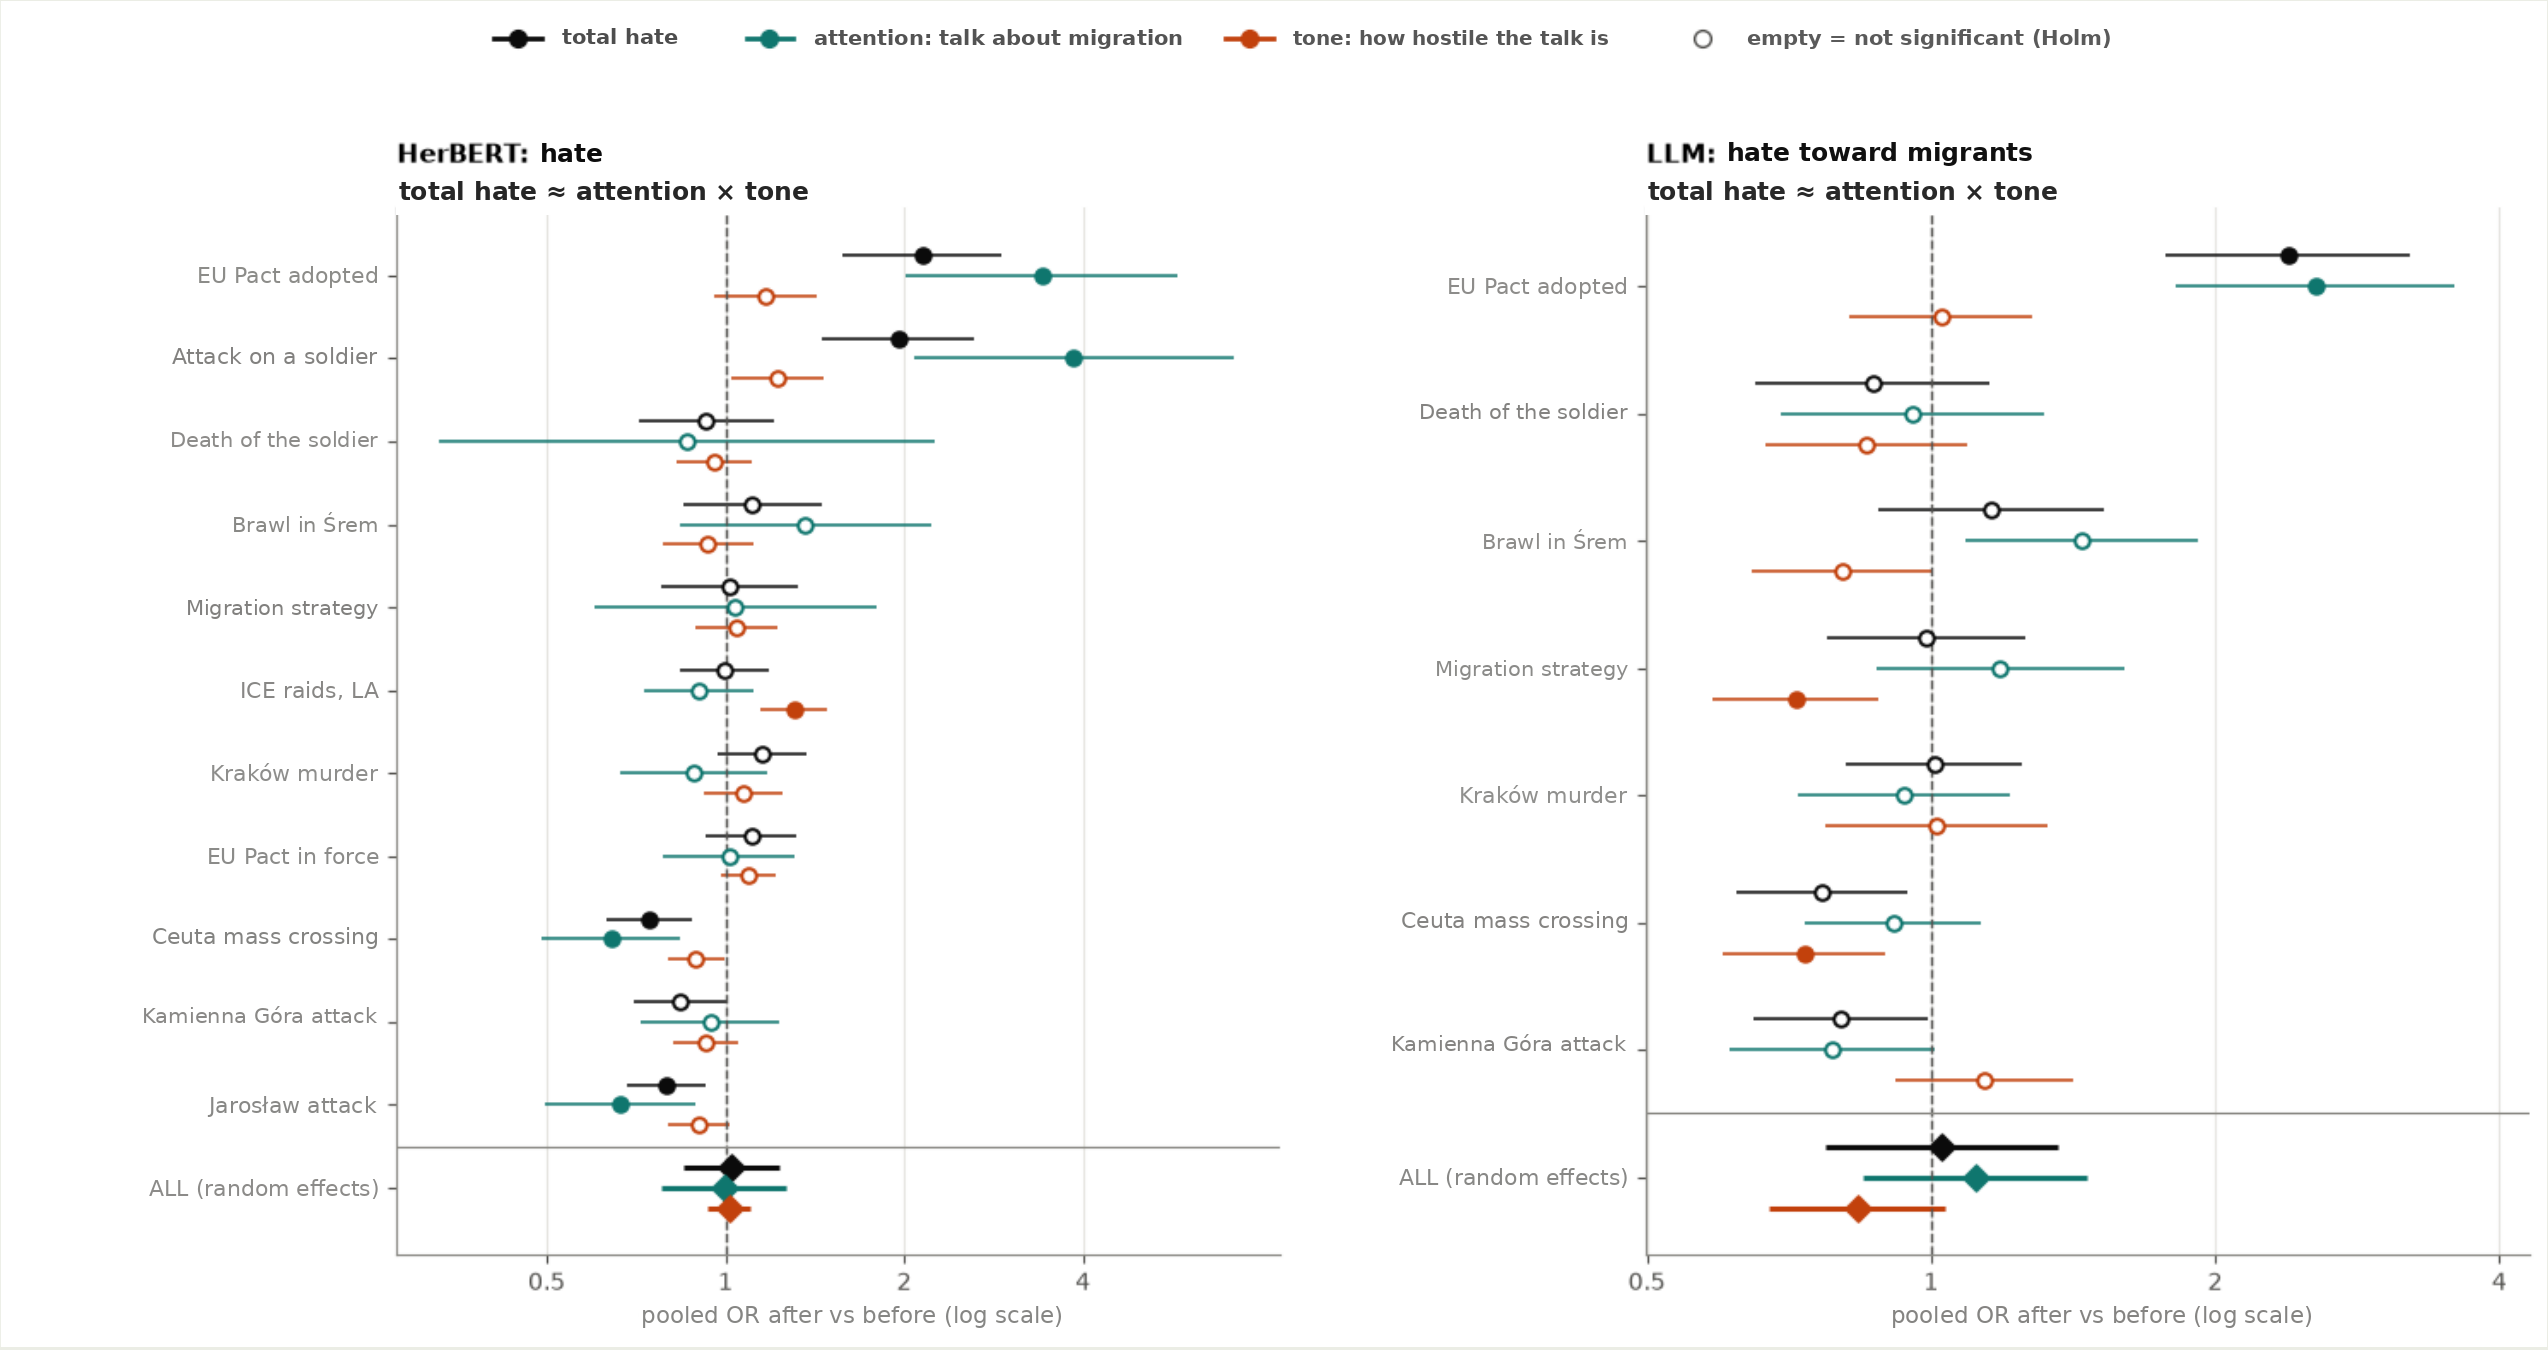
\includegraphics[width=0.85\textwidth]{fig_decomp_en.png}
  \caption{The change in hate (black) split into attention (teal: how much people write about migration) and tone (red: how hostile the discussion about migration is). Average OR per event with 95\% CI; empty points are not significant after Holm correction; bottom row: average over all events. Left: HerBERT; right: LLM.}
  \label{fig:decomp}
\end{figure*}


\howtoread{In Figure~\ref{fig:decomp}, if the black and teal points of an event are close together and the red point is near 1, hate grew only because more people wrote about migration, not because the discussion became more hostile.}

\paragraph{Hate grows because more people talk about migration.} Where hate changes, it follows attention (Figure~\ref{fig:decomp}). After the EU Pact, hate toward migrants increased with OR 2.39 and attention with OR 2.55, while the tone did not change (1.02). After the attack on the soldier, general hate increased 1.95-fold and attention 3.86-fold, with no significant change in tone (1.22). The decrease after Ceuta also followed attention (0.74 vs.\ 0.64). The only significant increase in tone was after the ICE raids in Los Angeles (1.30). \textbf{Events change how much people talk about migration, not how hostile they are.}

\paragraph{Timing.} After the EU Pact, hate on YouTube peaked at about six times the pre-event level on days 2--4 and returned to normal within a week, while on Wykop it doubled and stayed high for the whole period (Figure~\ref{fig:daily}). For Ceuta, the peak came \emph{before} day 0, so part of the ``decrease'' is a return to normal. After Kamienna Góra, hate on YouTube peaked with a delay, on day 9.

\begin{figure}[tbp]
  \centering
  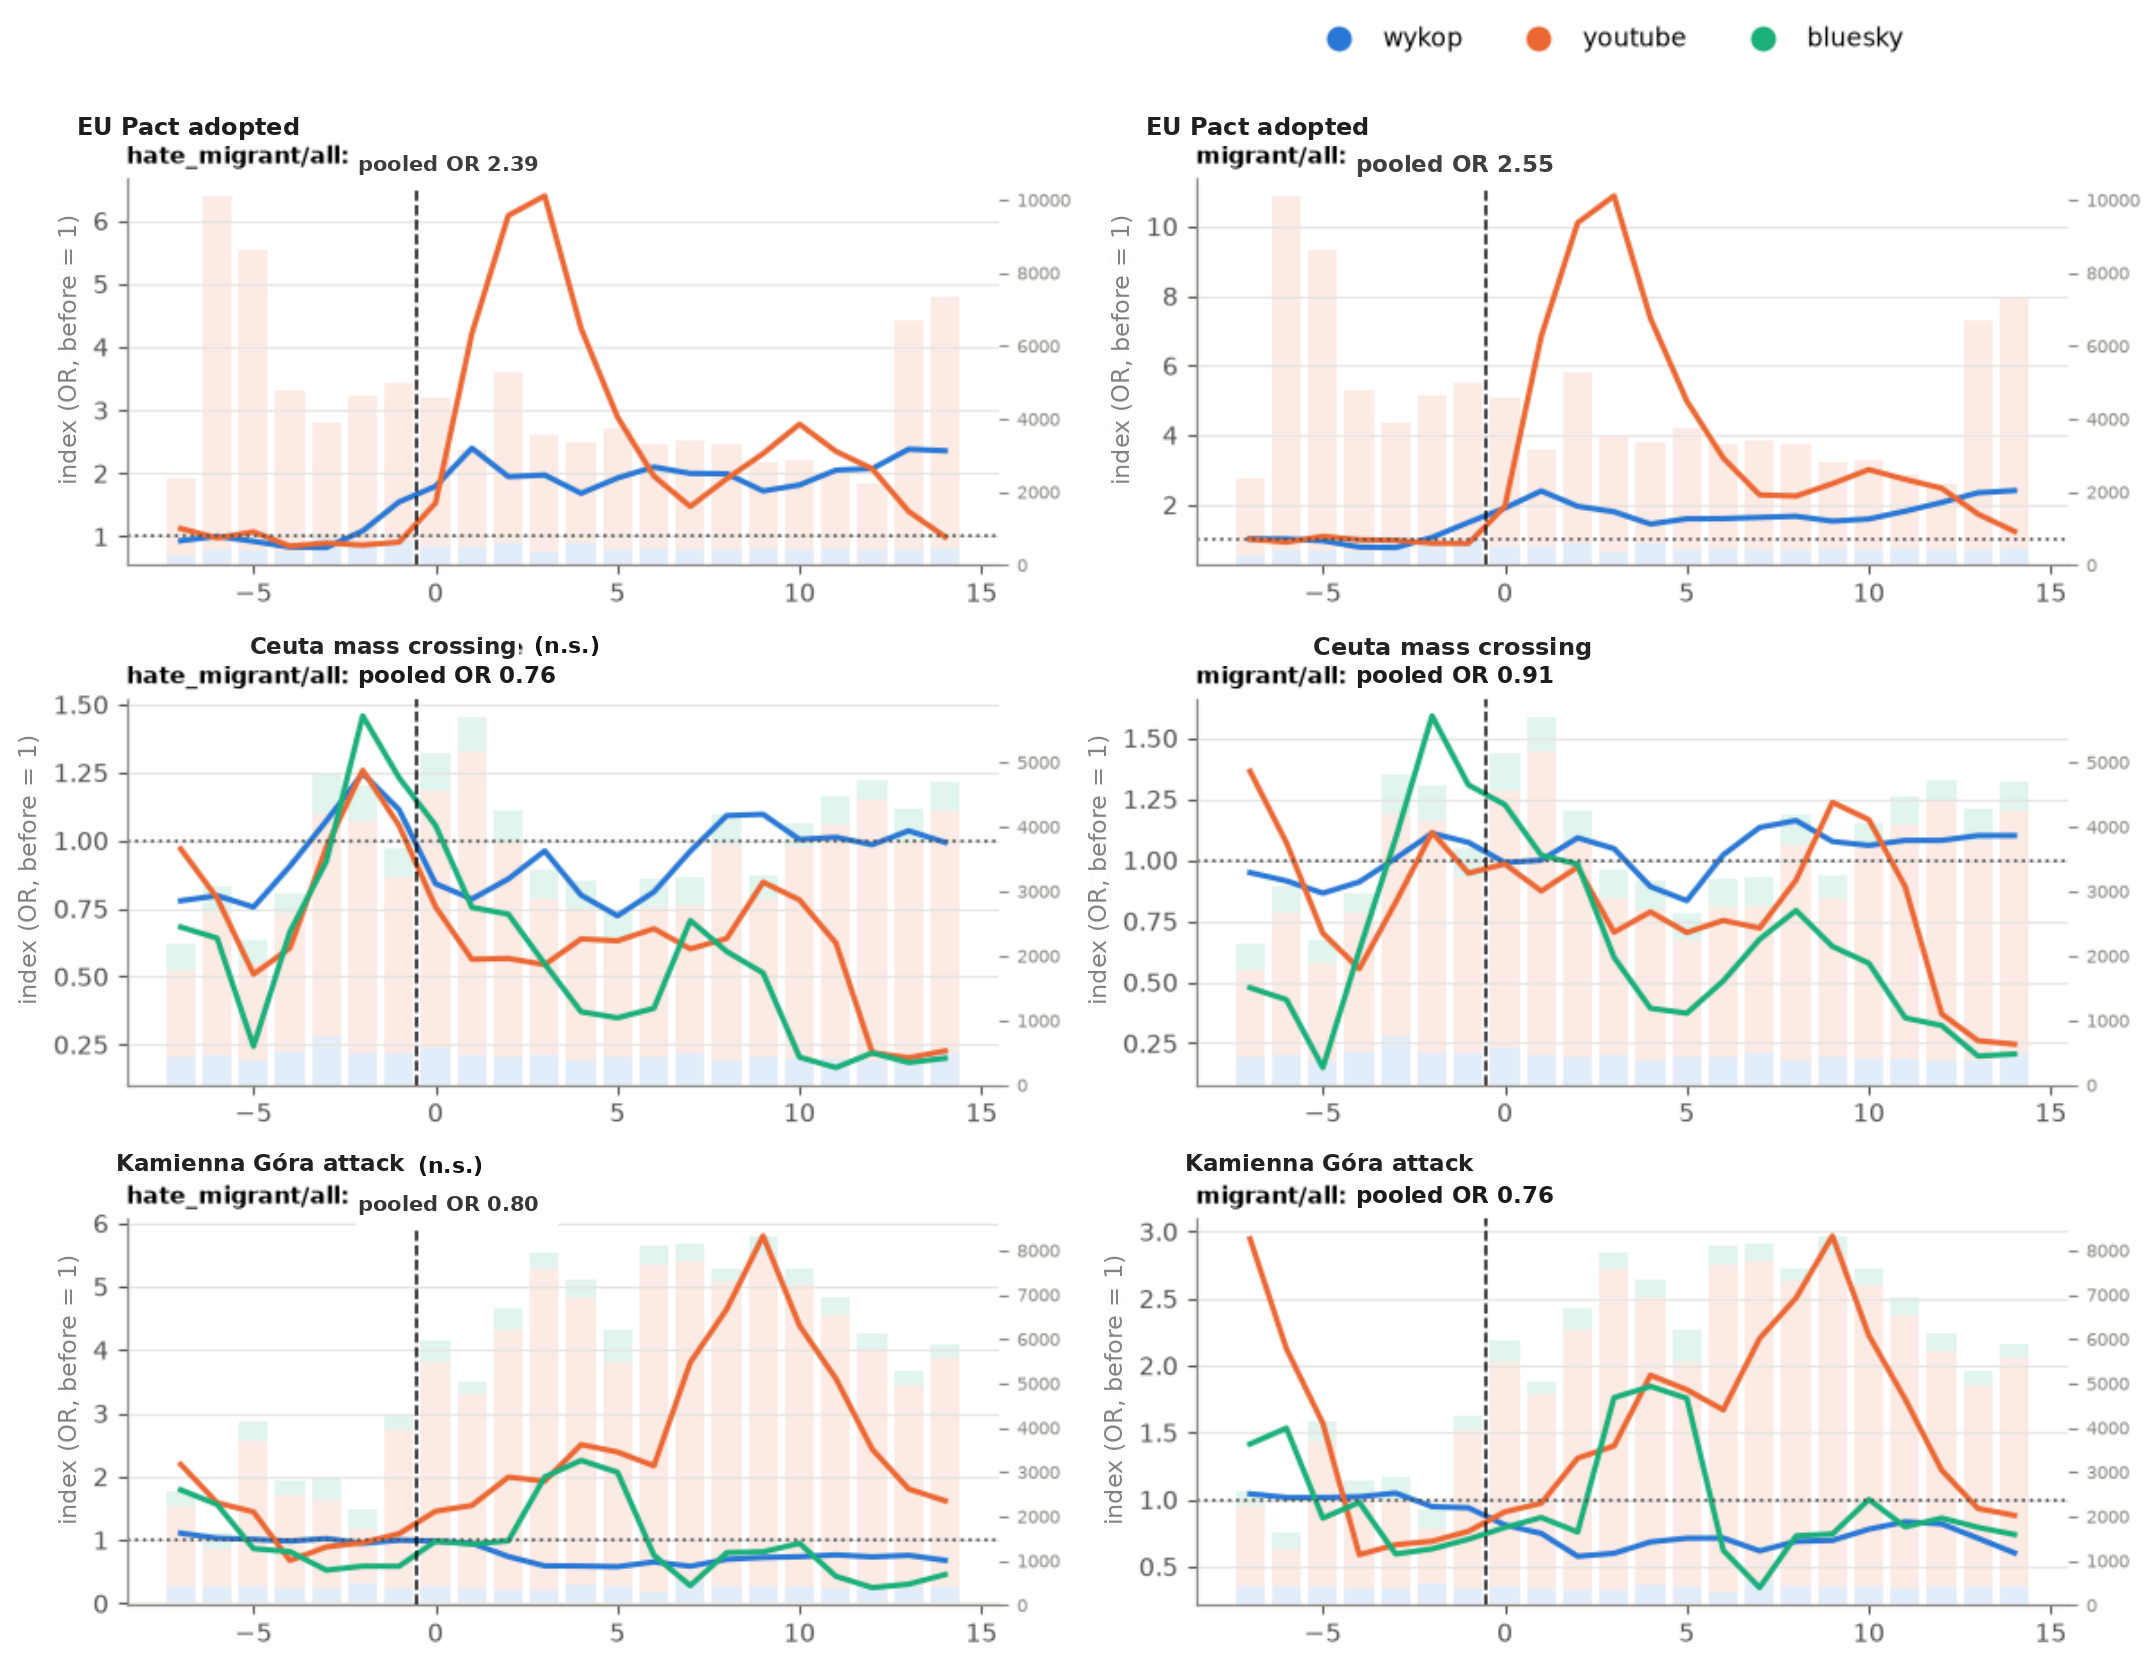
\includegraphics[width=\columnwidth]{fig_daily_en.png}
  \caption{Daily index of hate toward migrants (left) and of comments about migration (right), relative to the pre-event average (= 1), 3-day rolling mean. Bars: daily number of comments. Dashed line: day 0.}
  \label{fig:daily}
\end{figure}

\subsection{H2: Does the type of event matter?}

\begin{figure}[tbp]
  \centering
  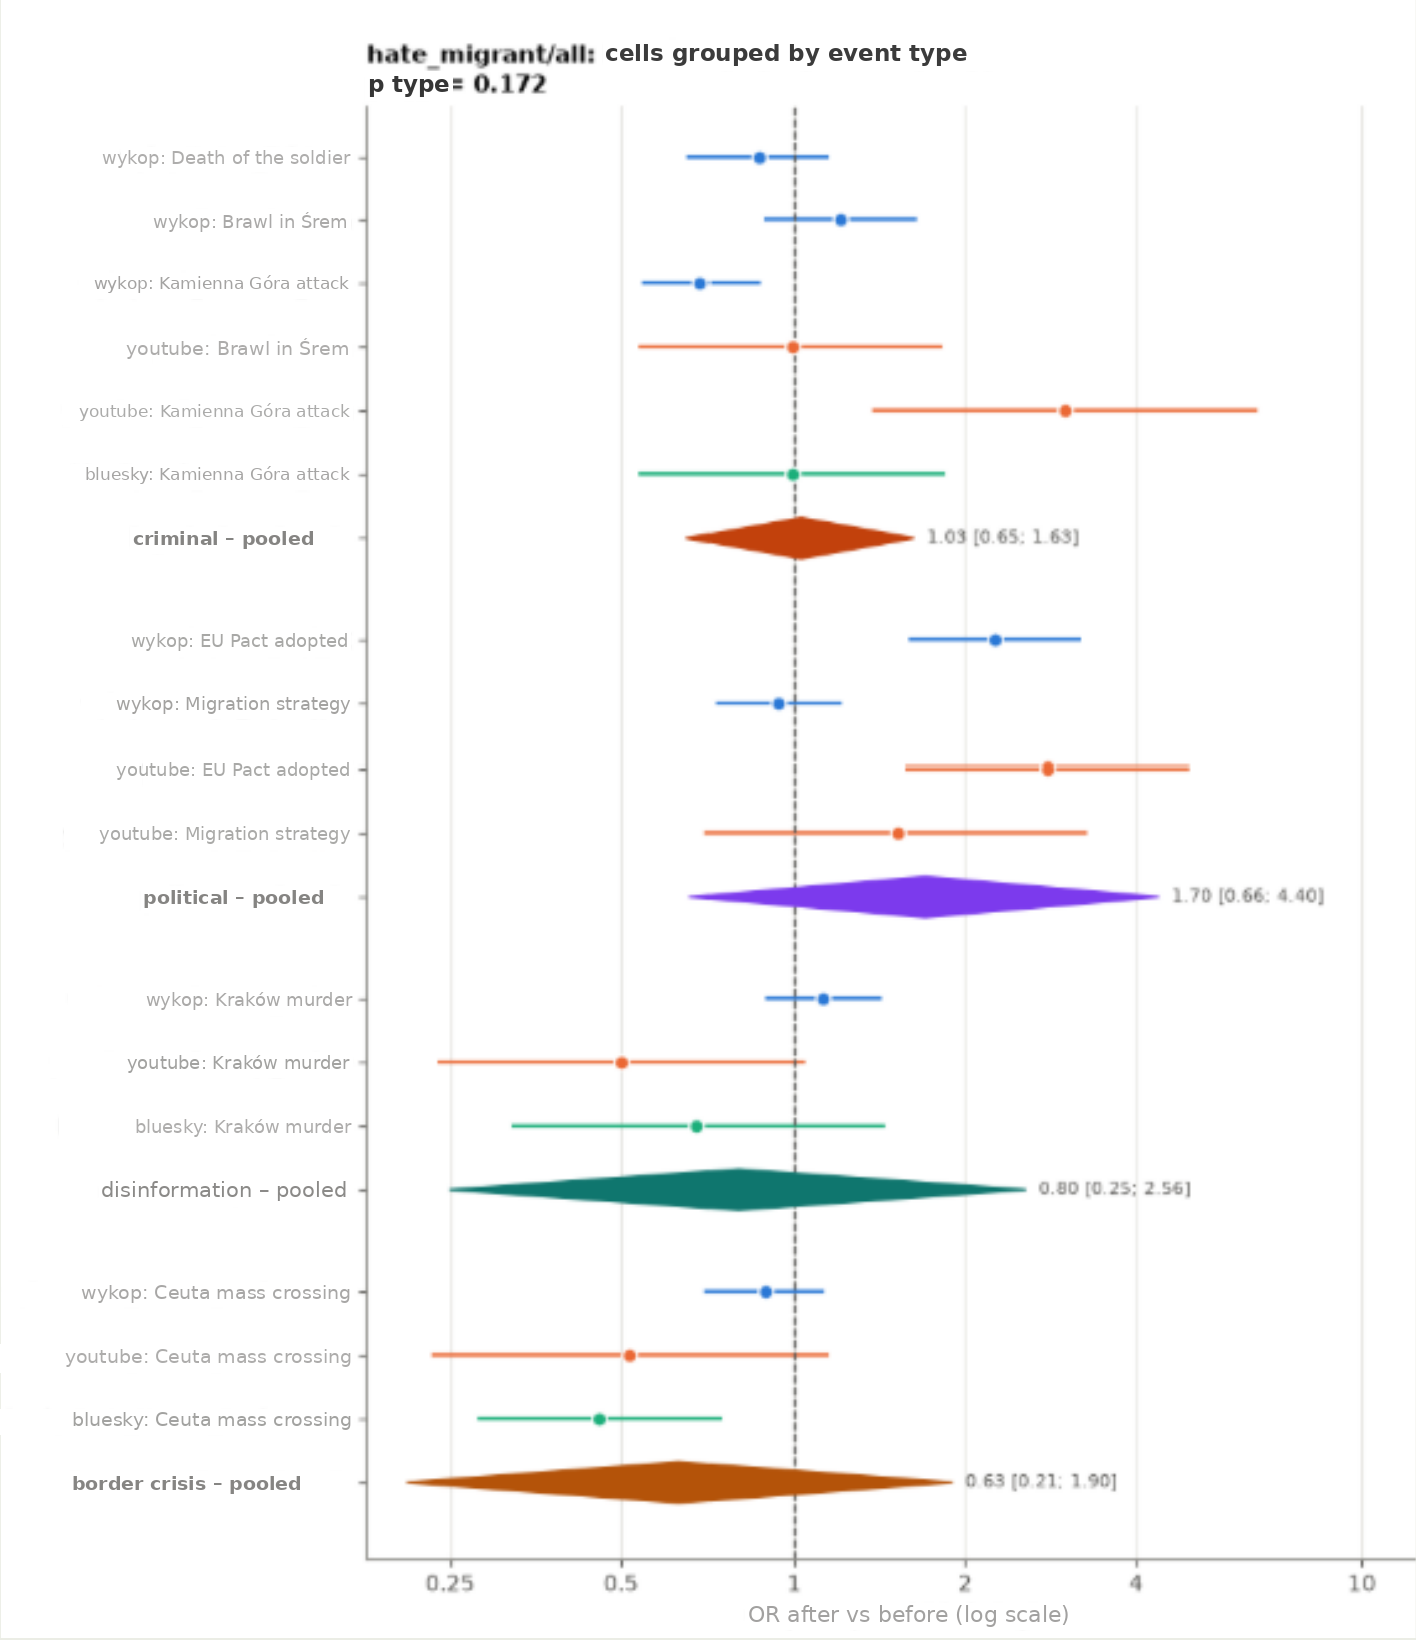
\includegraphics[width=0.9\columnwidth]{fig_h2_en.png}
  \caption{LLM cells grouped by event type, with the average OR per type (diamonds).}
  \label{fig:h2}
\end{figure}

\begin{table}[tbp]
\centering
\small
\setlength{\tabcolsep}{3pt}
\begin{tabular}{@{}lccc@{}}
\toprule
Type & H / L & HerBERT OR & LLM OR \\
\midrule
Criminal       & 5 / 3 & 1.05 [0.72, 1.56] & 1.03 [0.65, 1.63] \\
Political      & 4 / 2 & 1.17 [0.92, 1.50] & 1.70 [0.66, 4.40] \\
Disinformation & 1 / 1 & 0.92 [0.31, 2.72] & 0.80 [0.25, 2.56] \\
Border crisis  & 1 / 1 & 0.65 [0.24, 1.76] & 0.63 [0.21, 1.94] \\
\bottomrule
\end{tabular}
\caption{Average OR by event type. H / L: number of events in the HerBERT / LLM analysis.}
\label{tab:h2}
\end{table}

Political events show the largest average increase, but this is driven by the EU Pact, while the migration strategy hardly changed hate. Criminal events average OR $\approx$ 1, with cells going in opposite directions (Figure~\ref{fig:h2}, Table~\ref{tab:h2}). Disinformation and the border crisis point downward, but their confidence intervals include 1. The type of event does not explain the differences: meta-regression $F = 1.08$ (HerBERT) and $2.03$ (LLM), permutation $p = 0.53$ and $0.29$. \textbf{H2 is not supported}: the size of the reaction depends on the specific event and platform, not on its type. With only one event of some types, this test has little power.

\subsection{H3: Do platforms react differently?}

\begin{figure*}[t]
  \centering
  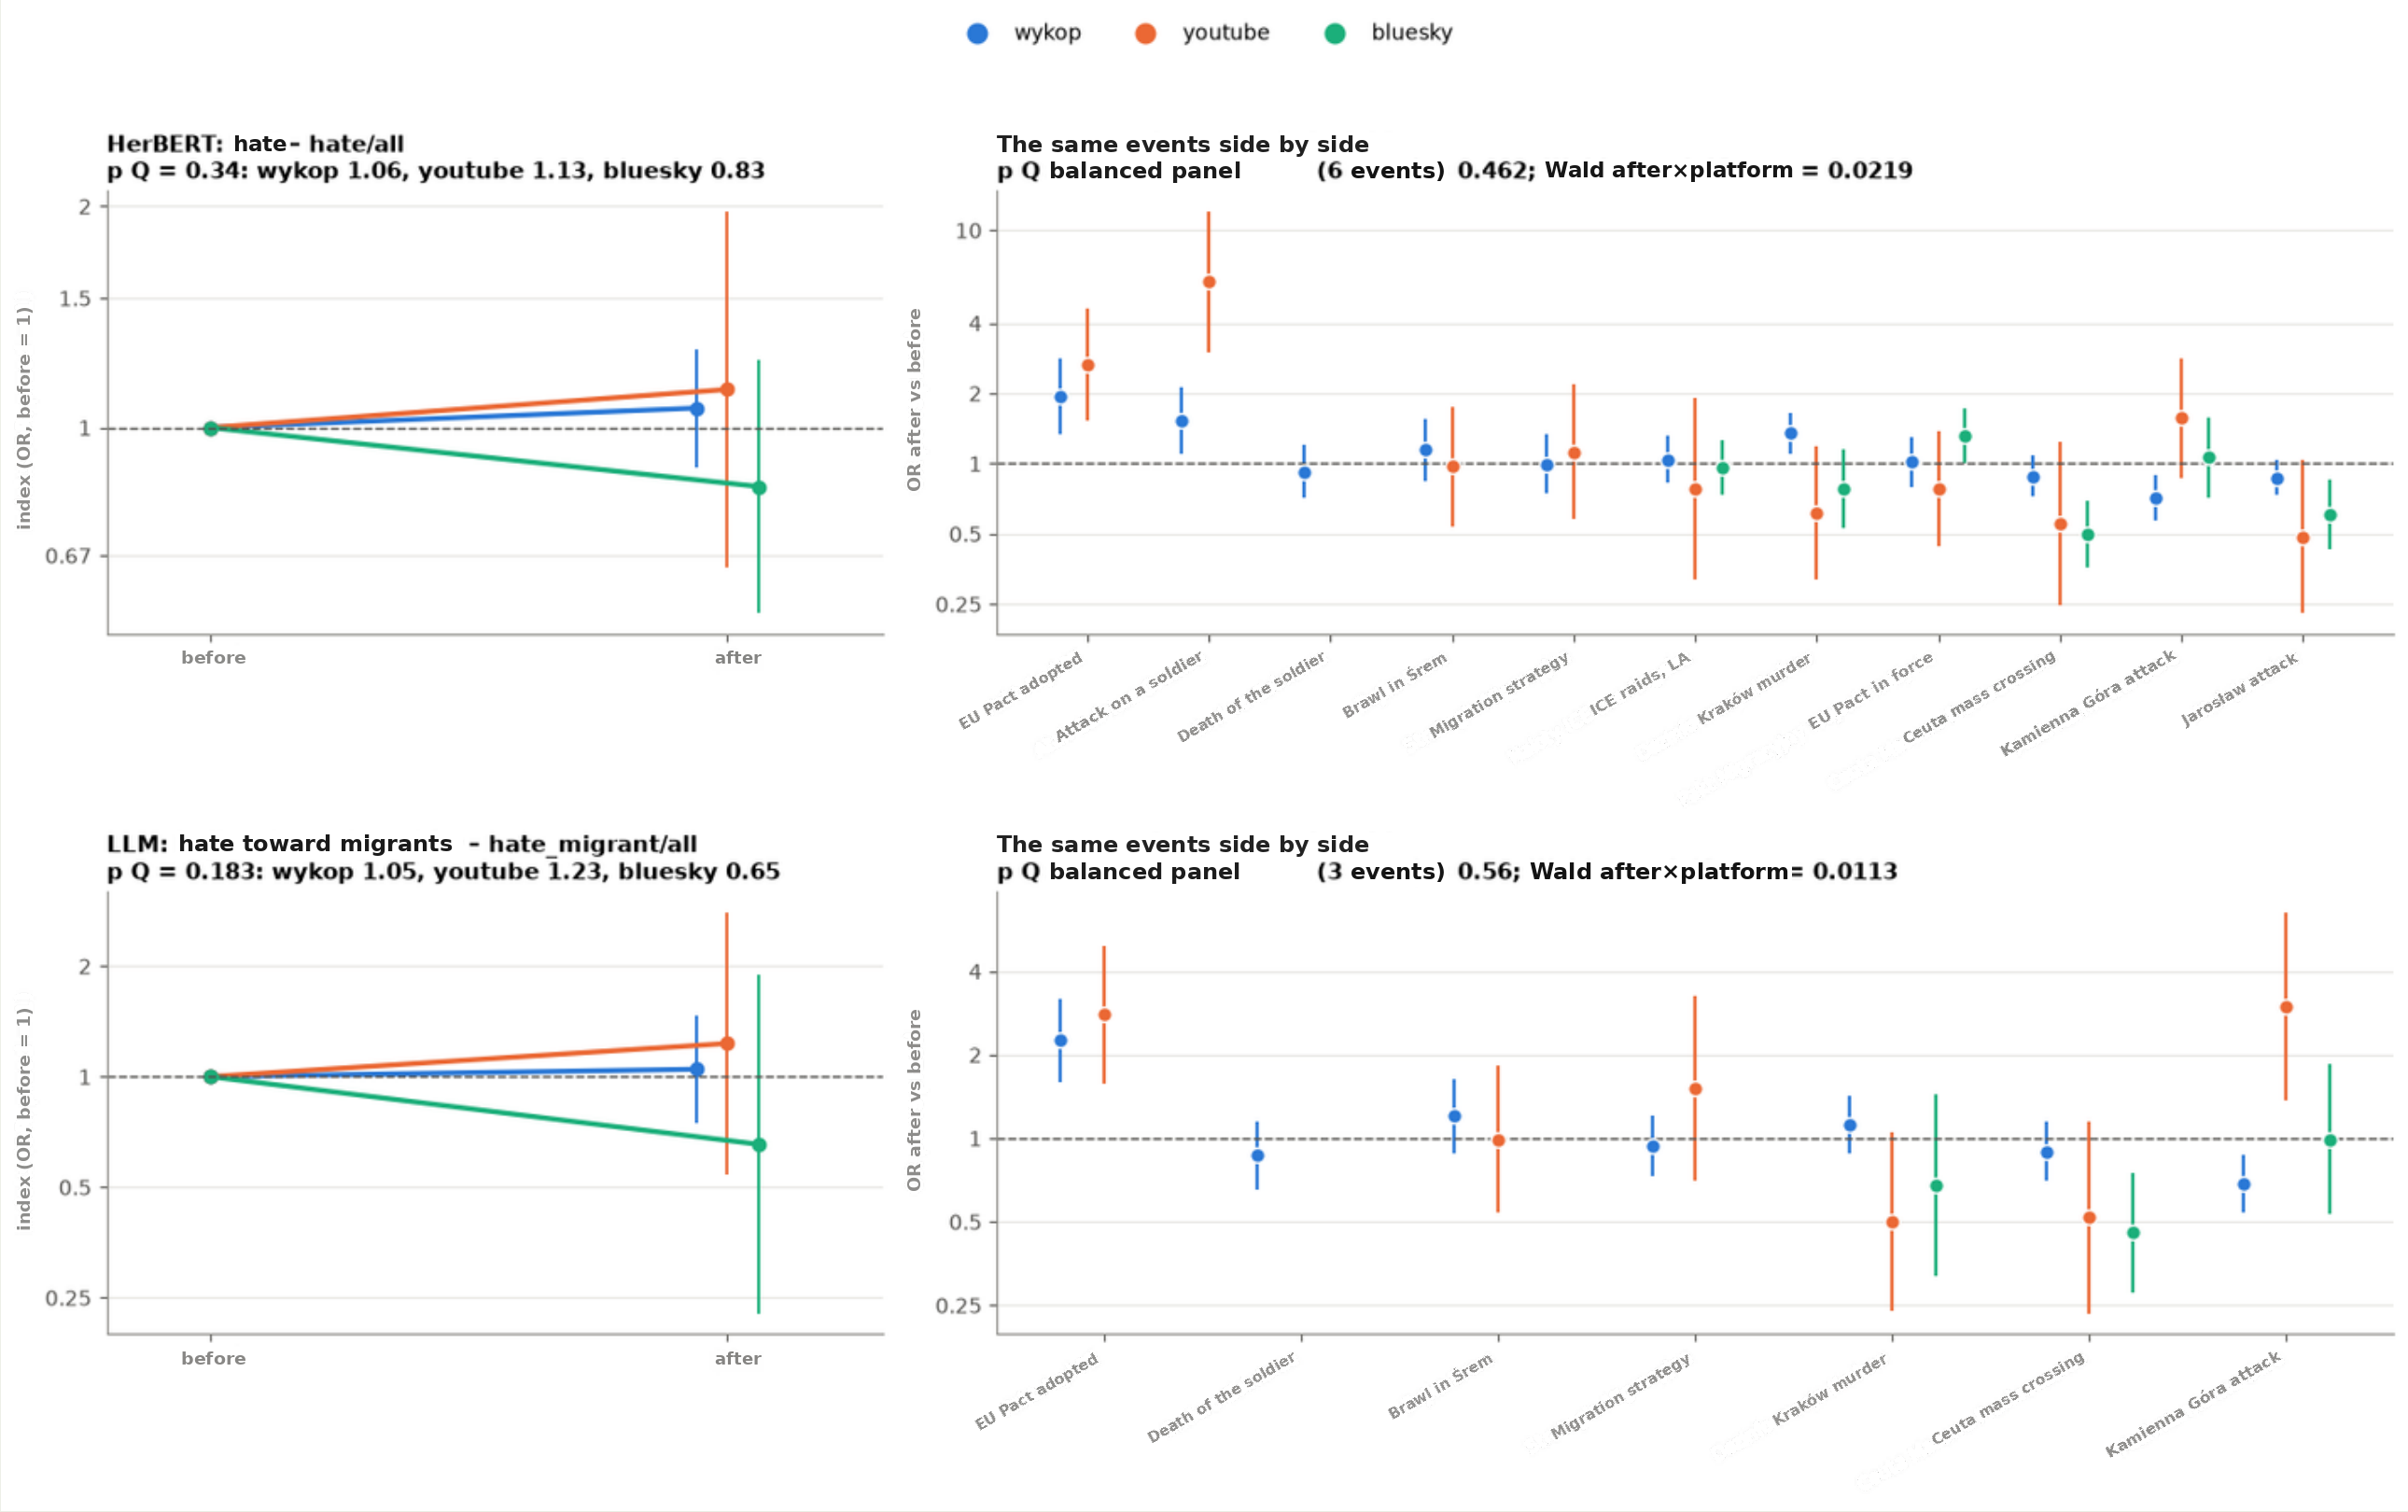
\includegraphics[width=0.85\textwidth]{fig_h3_en.png}
  \caption{Platforms. Left: average OR per platform shown as a change from ``before'' (= 1) to ``after'', with 95\% CI. Right: the same events side by side on each platform. Top: HerBERT; bottom: LLM.}
  \label{fig:h3}
\end{figure*}


\howtoread{In the right panels of Figure~\ref{fig:h3}, platforms reacted differently to an event if their points lie on different sides of the line at 1 and their intervals do not overlap.}

The average ORs point in different directions: Wykop 1.06 (HerBERT) / 1.05 (LLM), YouTube 1.13 / 1.23 and Bluesky 0.83 / 0.65 (Figure~\ref{fig:h3}). These differences are not significant ($Q = 2.16$, $p = 0.34$; $Q = 3.39$, $p = 0.18$), also on the balanced panel ($p = 0.46$ and $0.56$). The interaction in the comment-level model is significant ($p = 0.022$ and $0.011$), but not when only events common to all platforms are used ($p = 0.11$ for both). The platforms differ much more in the \emph{level} of hate -- among topic-filtered comments, HerBERT labels 44\% as hateful on YouTube, 34\% on Wykop and 20\% on Bluesky -- than in their \emph{reaction} to events. \textbf{H3 is partially supported}: the directions differ, but the differences are not robust.

\begin{table}[tbp]
\centering
\small
\setlength{\tabcolsep}{2.5pt}
\begin{tabular}{@{}p{0.9cm}p{2.9cm}p{2.9cm}@{}}
\toprule
 & HerBERT (\texttt{hate}) & LLM (\texttt{hate\_migrant}) \\
\midrule
H1 & partially; OR 1.03 [0.85, 1.23], $p = 0.79$ & partially; OR 1.03 [0.77, 1.36], $p = 0.85$ \\
H2 & not supported; $F = 1.08$, $p_\text{perm} = 0.53$ & not supported; $F = 2.03$, $p_\text{perm} = 0.29$ \\
H3 & partially; $Q = 2.16$, $p_\text{panel} = 0.46$ & partially; $Q = 3.39$, $p_\text{panel} = 0.56$ \\
\bottomrule
\end{tabular}
\caption{Summary of the hypothesis tests.}
\label{tab:summary}
\end{table}

\subsection{Q1: What is hate toward migrants about?}

\begin{figure}[tbp]
  \centering
  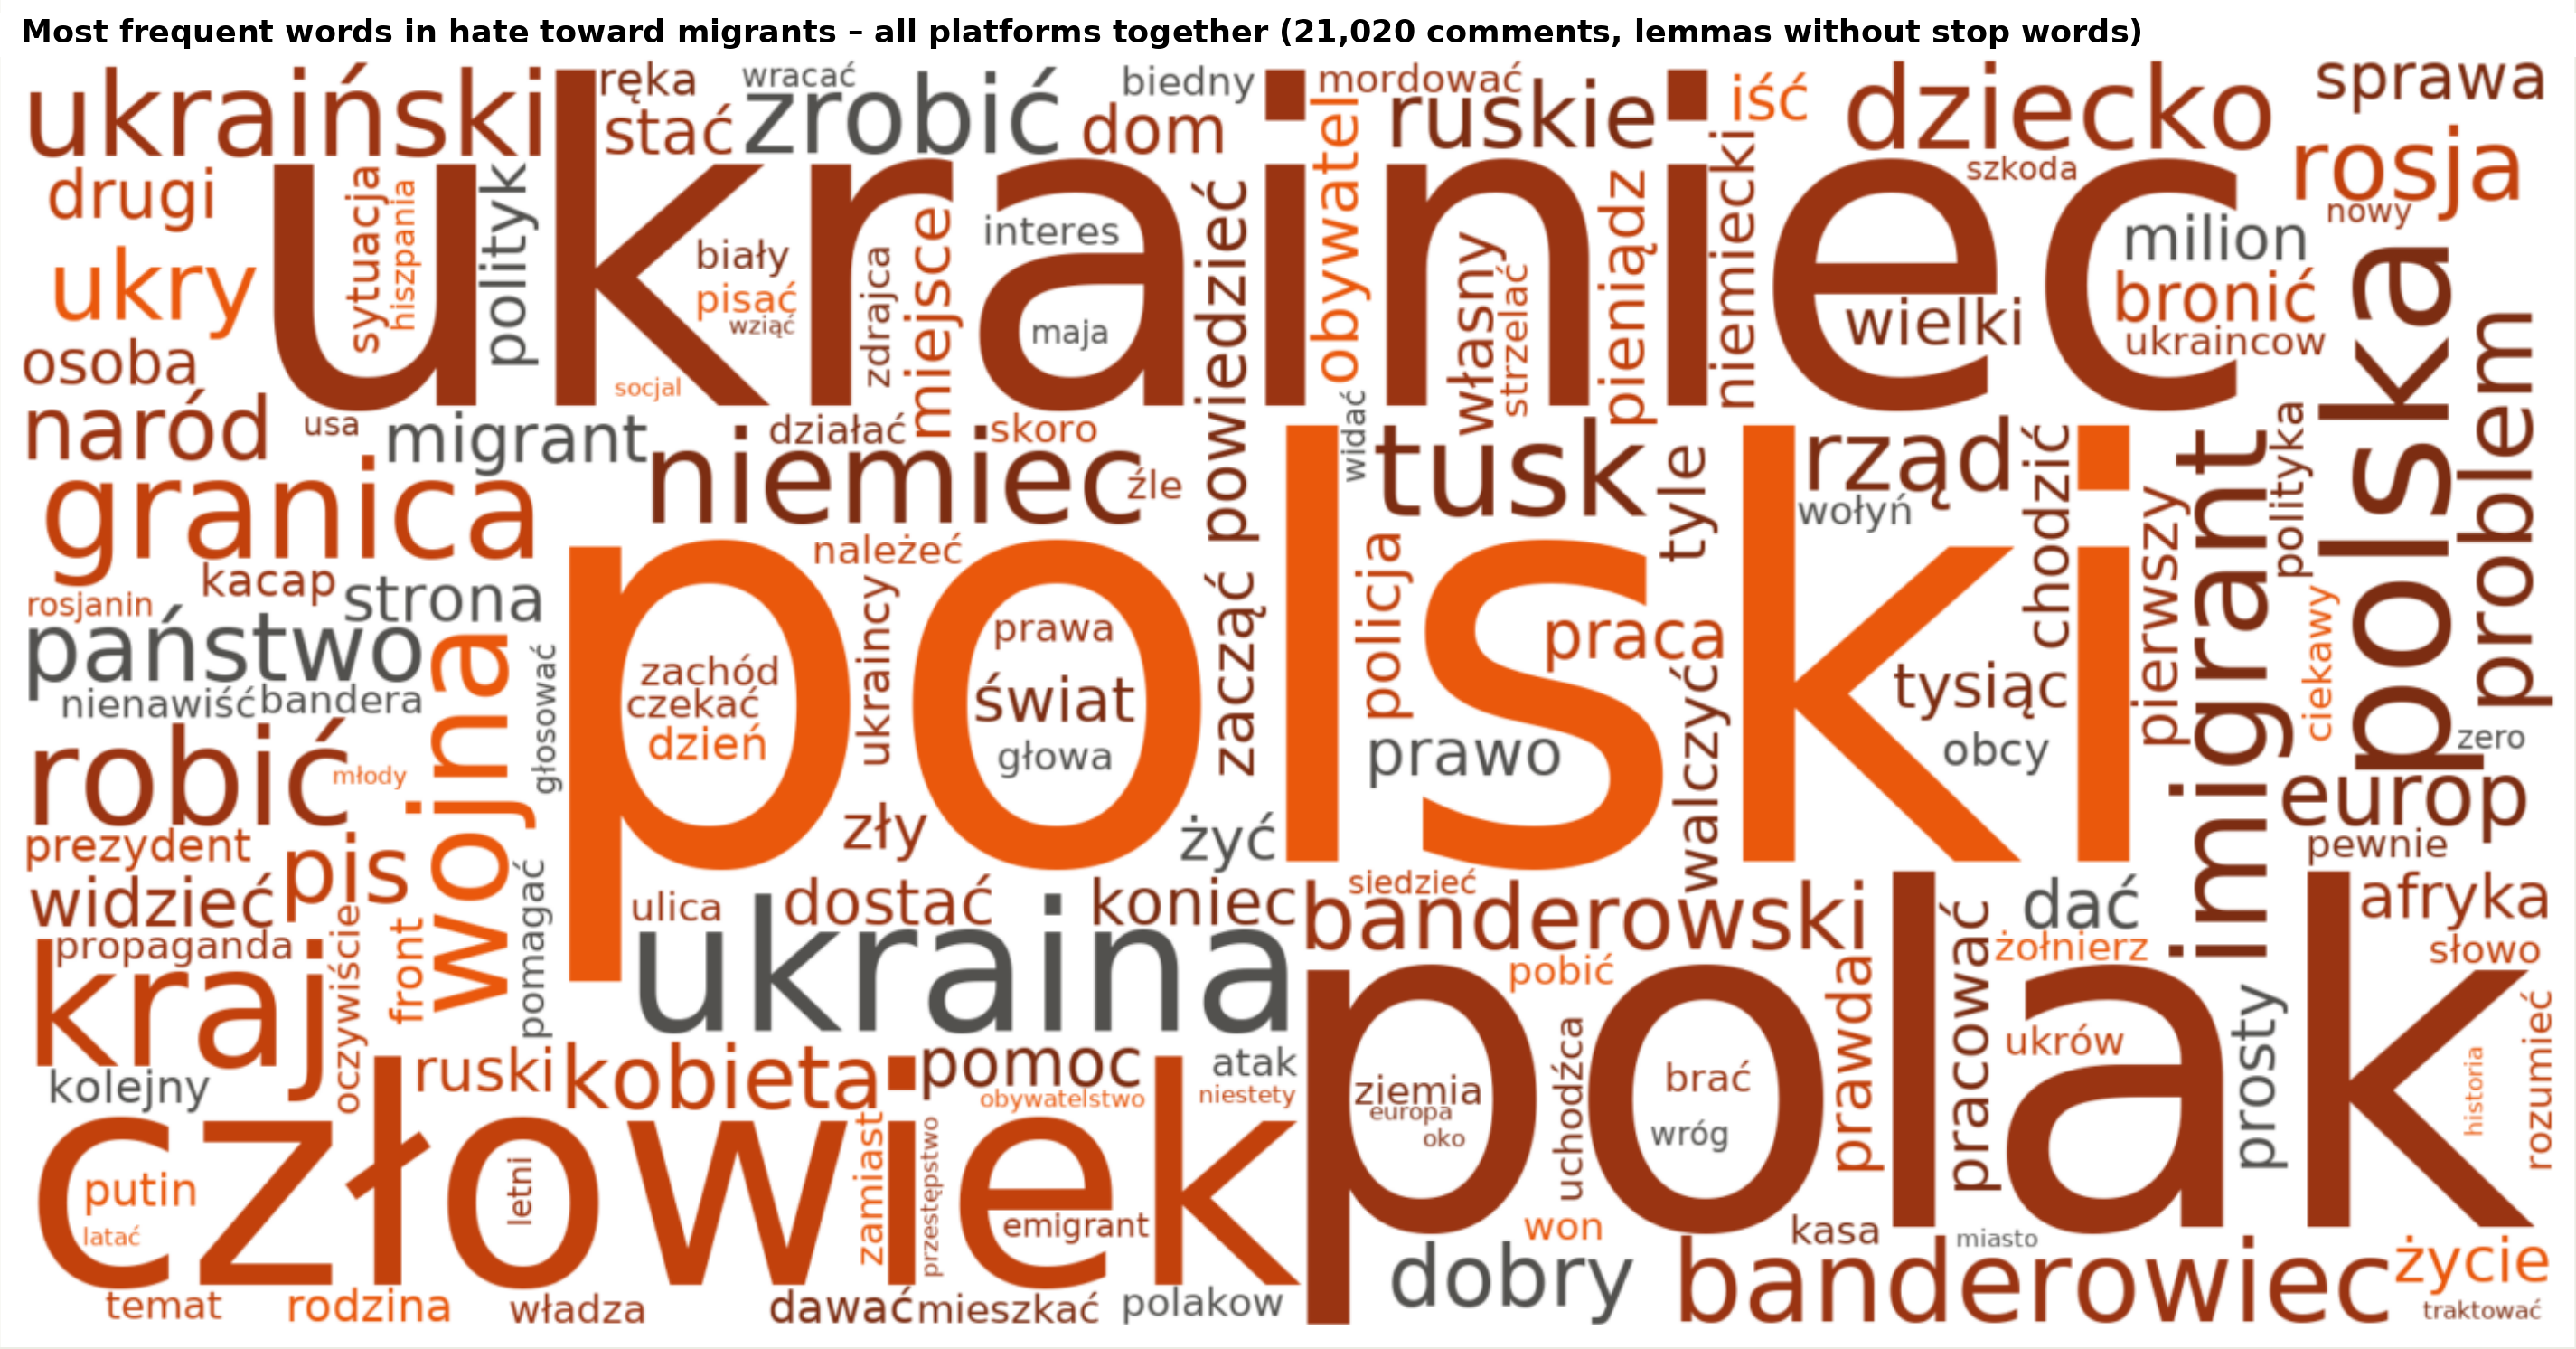
\includegraphics[width=\columnwidth]{fig_cloud_en.png}
  \caption{Most frequent words in hate toward migrants, all platforms together (21,020 comments labelled \texttt{hate\_migrant}; Polish lemmas, stop words removed). Larger words are more frequent.}
  \label{fig:cloud}
\end{figure}

\begin{figure*}[t]
  \centering
  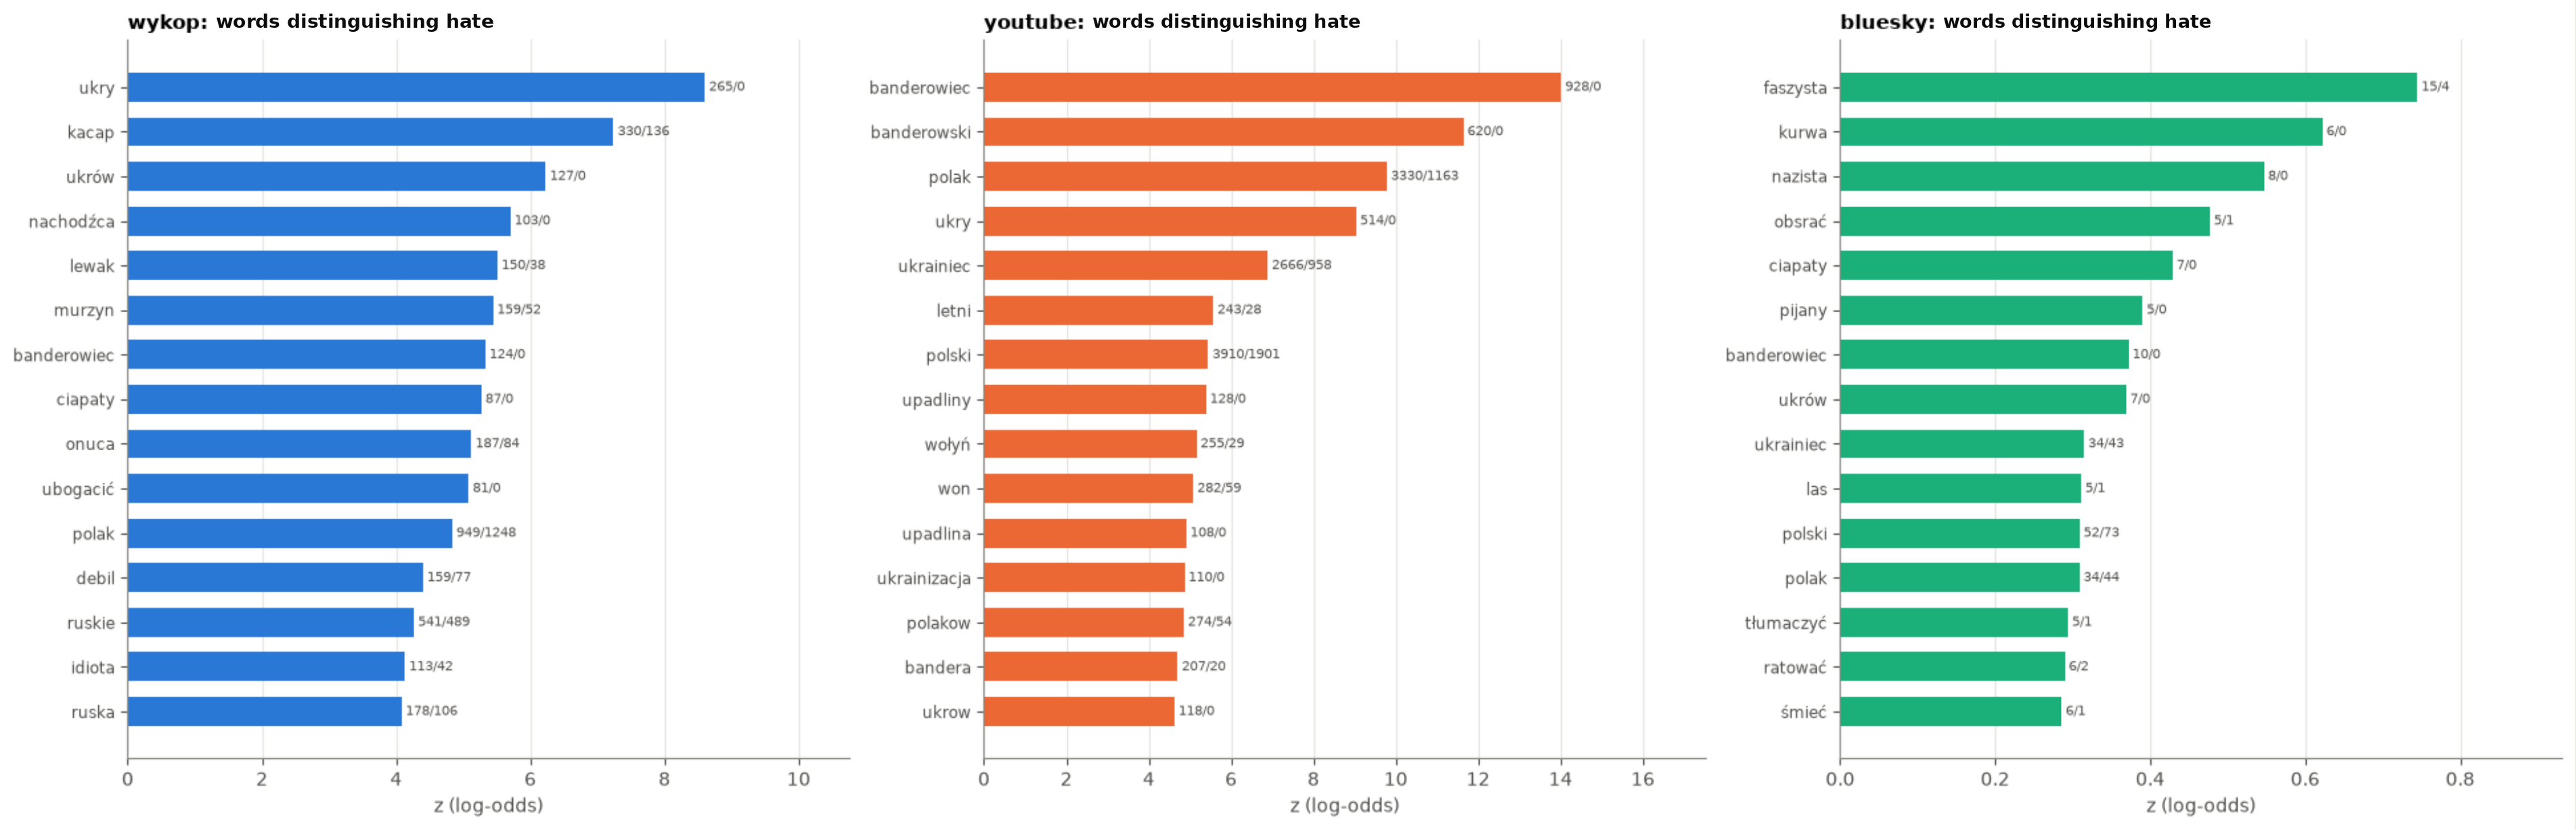
\includegraphics[width=0.95\textwidth]{fig_words_en.png}
  \caption{Words that most clearly distinguish hate toward migrants from other comments about migration, per platform (weighted log-odds $z$; numbers: occurrences in hateful / other comments). Words are Polish lemmas, e.g.\ \textit{ukry} and \textit{banderowiec} -- slurs for Ukrainians, \textit{kacap} -- a slur for Russians, \textit{nachodźca} -- a slur for refugees.}
  \label{fig:words}
\end{figure*}


\begin{figure*}[t]
  \centering
  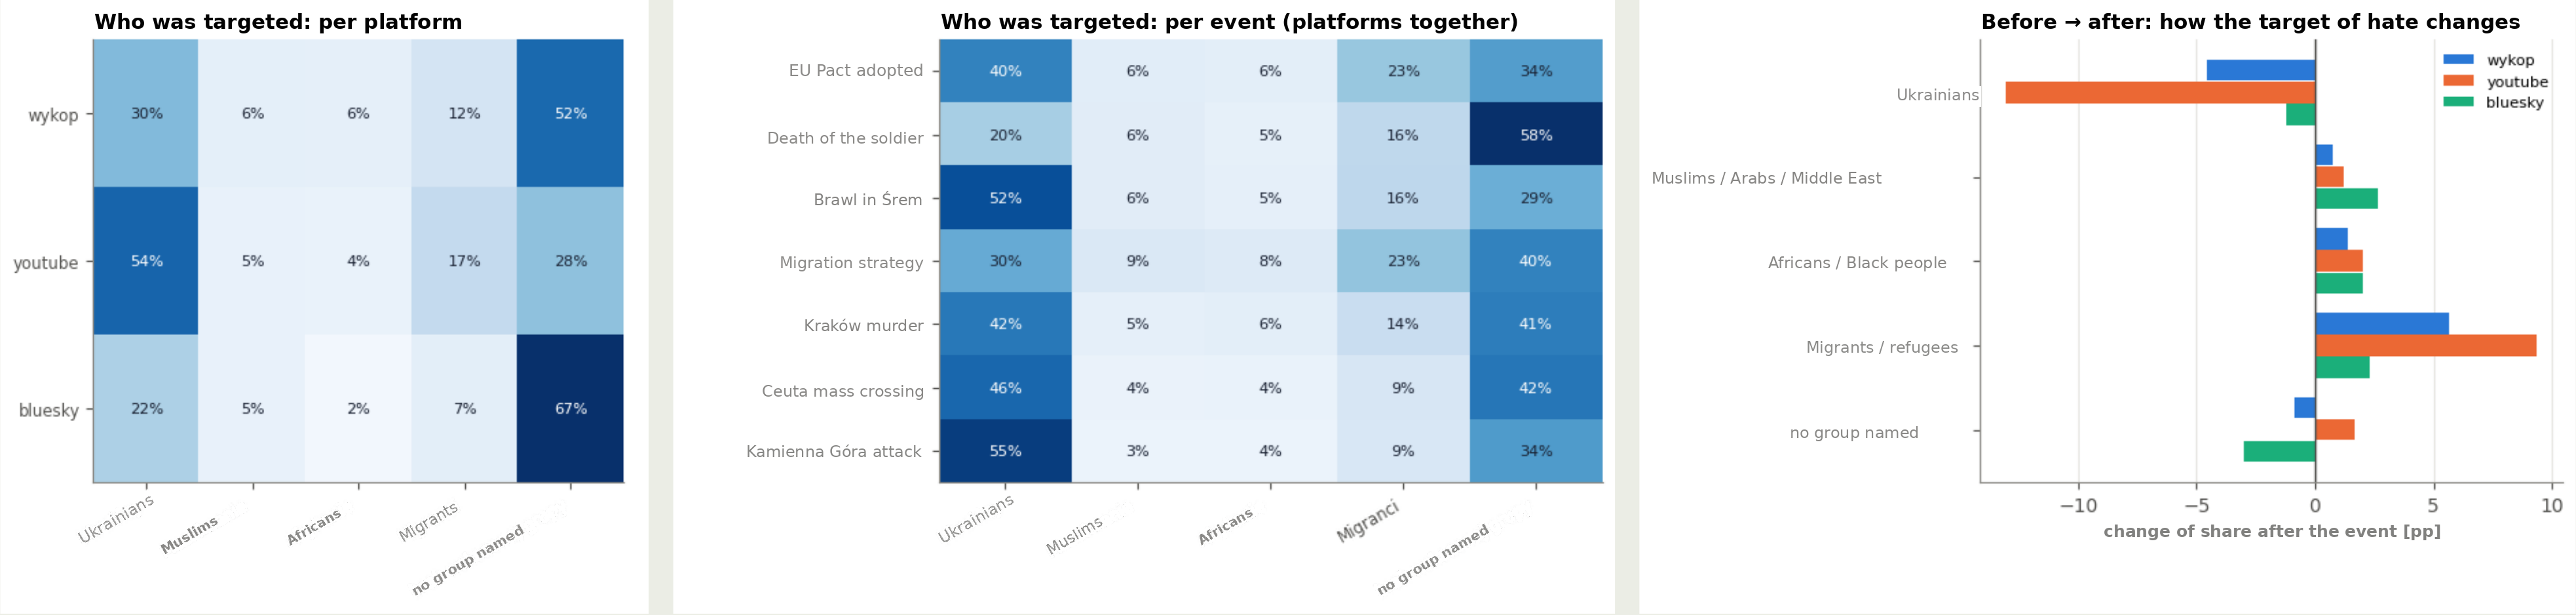
\includegraphics[width=0.92\textwidth]{fig_targets_en.png}
  \caption{Targets of hate toward migrants, found with keyword lists. Left: share of hateful comments that mention each group, per platform (Ukrainians, Muslims, Africans, migrants in general, no group named). Middle: per event. Right: change of the share after the event, in percentage points. One comment can mention several groups.}
  \label{fig:targets}
\end{figure*}

\paragraph{Words.} Among the 21,020 comments labelled \texttt{hate\_migrant}, the most frequent words (Figure~\ref{fig:cloud}) refer to Ukrainians (\textit{Ukrainiec}, \textit{Ukraina}, \textit{banderowiec}, the slur \textit{ukry}) and, almost as often, to Poles (\textit{Polak}, \textit{polski}), which suggests an ``us versus them'' framing. Politicians (Tusk), parties and other countries (Germany, Russia) are also frequent. The words that most clearly distinguish hate from other comments about migration (Figure~\ref{fig:words}) are ethnic slurs together with general insults on Wykop (\textit{ukry}, \textit{nachodźca}, \textit{ciapaty}, \textit{lewak}, \textit{debil}), and almost exclusively anti-Ukrainian words with historical references on YouTube (\textit{banderowiec}, \textit{upadlina}, \textit{Wołyń}, \textit{ukrainizacja}, \textit{won}). On Bluesky the counts are too small to draw conclusions.


\paragraph{Targets.} Ukrainians are the most frequently named target (54\% of hate toward migrants on YouTube, 30\% on Wykop, 22\% on Bluesky); Muslims and Africans account for a few per cent each (Figure~\ref{fig:targets}). Much hate does not name any group directly (up to 67\% on Bluesky), and some of it is probably also about Ukrainians. After events, the share of hate aimed at Ukrainians \emph{falls} (by about 13 percentage points on YouTube), and the share aimed at migrants in general grows (by about 9 points). Several events -- the EU Pact, the migration strategy, the death of the soldier, Ceuta -- concerned migrants from outside Ukraine, and discussions about them use general words such as ``immigrants'' or ``illegals''. Hate toward Ukrainians does not disappear; it becomes a smaller part of all hate.

\paragraph{Authors and likes.} Ordinary discussion is concentrated: on Wykop, the 20\% most active authors write about 70\% of comments about migration (Gini 0.65; Bluesky 0.68). Hate is spread more evenly (Gini 0.43 and 0.36): the 20\% most active haters write about half of it (Figure~\ref{fig:authors}). \textbf{Hate toward migrants is written by many occasional users, not by a few accounts.} Hate is not always rewarded: it receives about one third more likes than other comments on Bluesky ($\times$1.33), about half as many on YouTube ($\times$0.52), and a similar number on Wykop ($\times$1.11, not significant).

\begin{figure}[tbp]
  \centering
  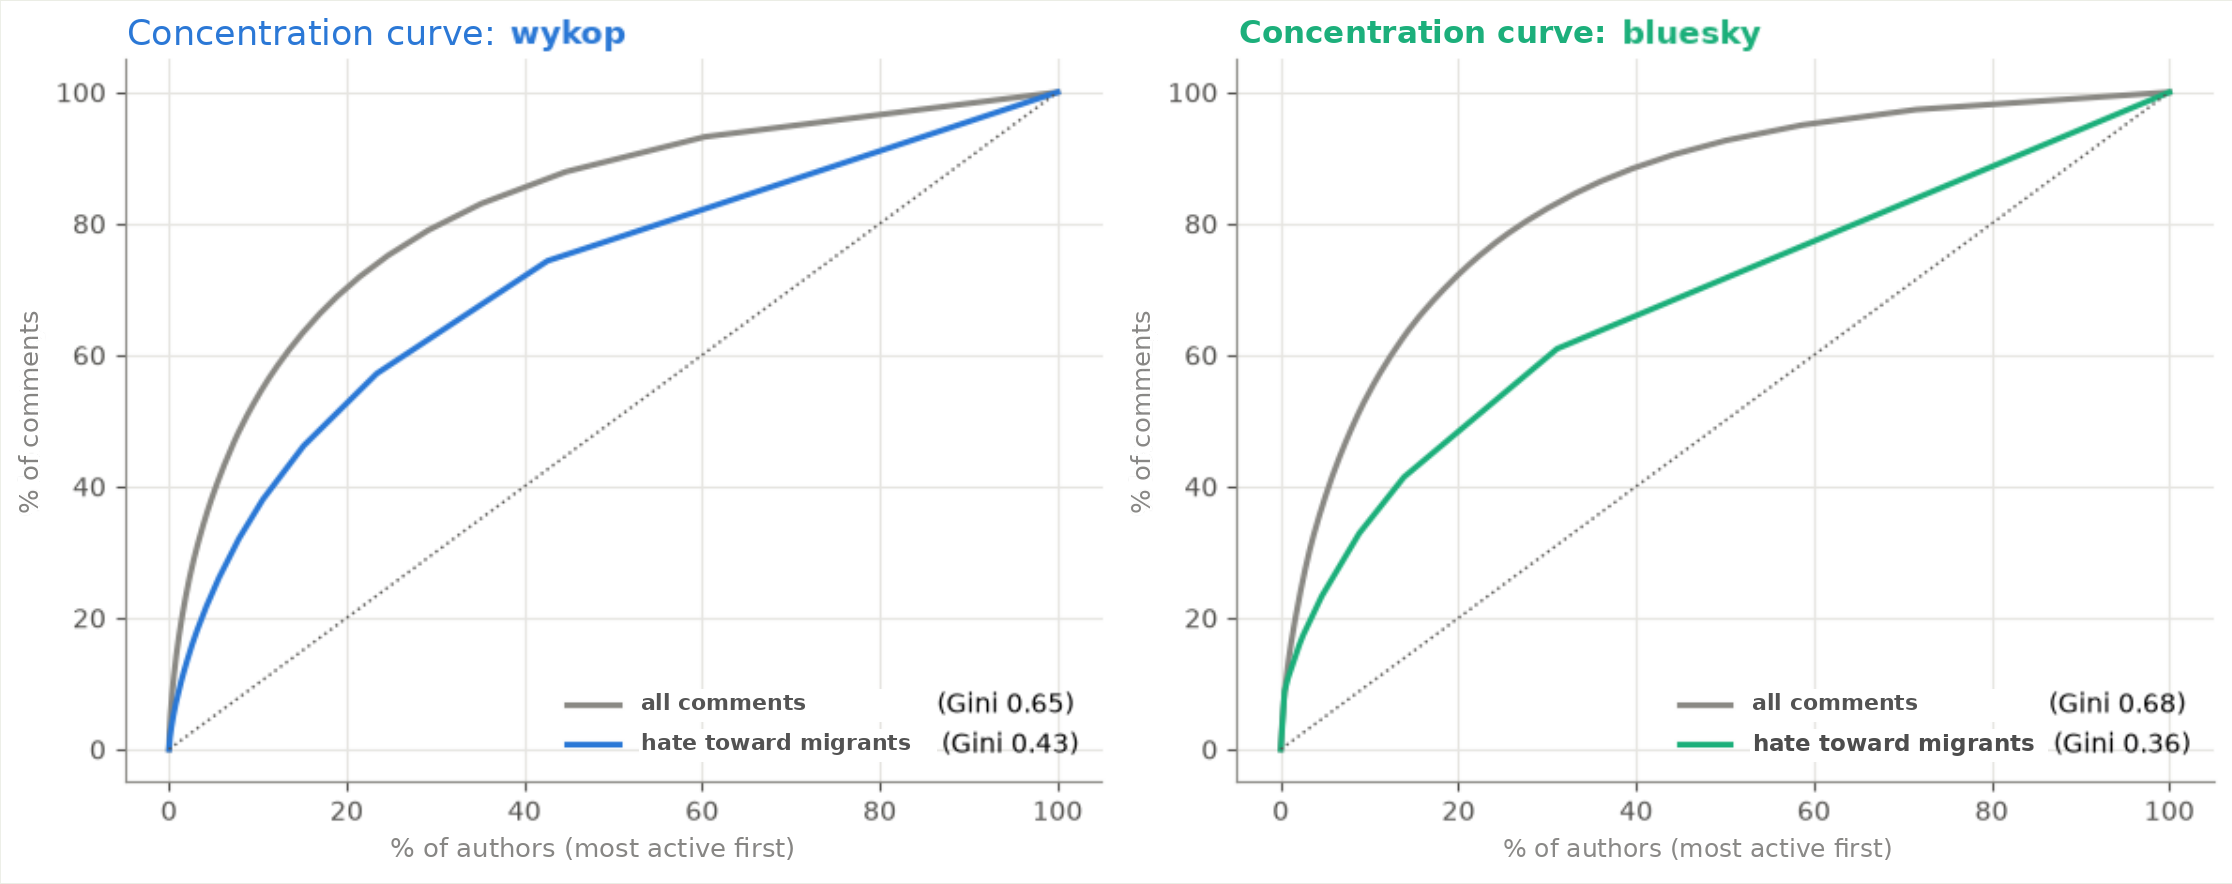
\includegraphics[width=\columnwidth]{fig_authors_en.png}\\[3pt]
  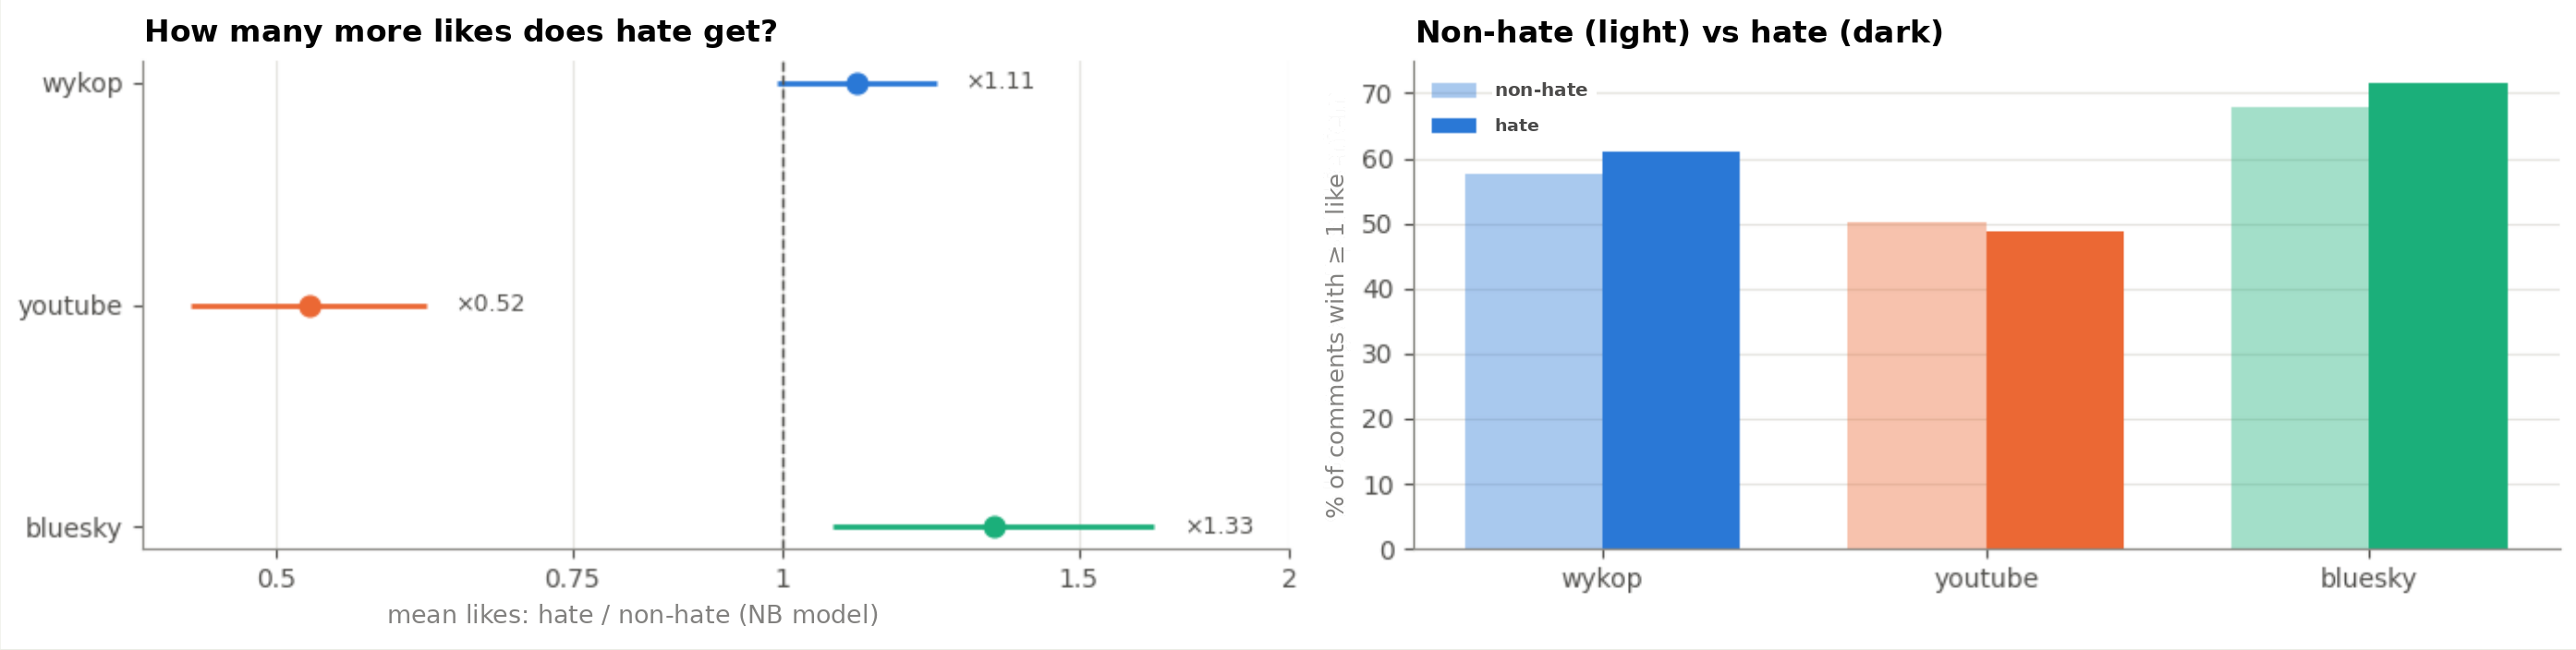
\includegraphics[width=\columnwidth]{fig_likes_en.png}
  \caption{Top: concentration curves for Wykop and Bluesky. Authors are sorted from the most active; the curve shows what share of comments they wrote (grey: all comments about migration; colour: hate toward migrants). Bottom: ratio of mean likes of hateful to other comments (negative binomial model, 95\% CI) and share of comments with at least one like. YouTube data contain no author identifiers.}
  \label{fig:authors}
\end{figure}

\howtoread{The further a curve in Figure~\ref{fig:authors} lies above the diagonal, the more the writing is concentrated in a few hands. The Gini coefficient summarises this: 0 means that everyone writes the same amount, 1 that one person writes everything.}

\begin{figure*}[t]
  \centering
  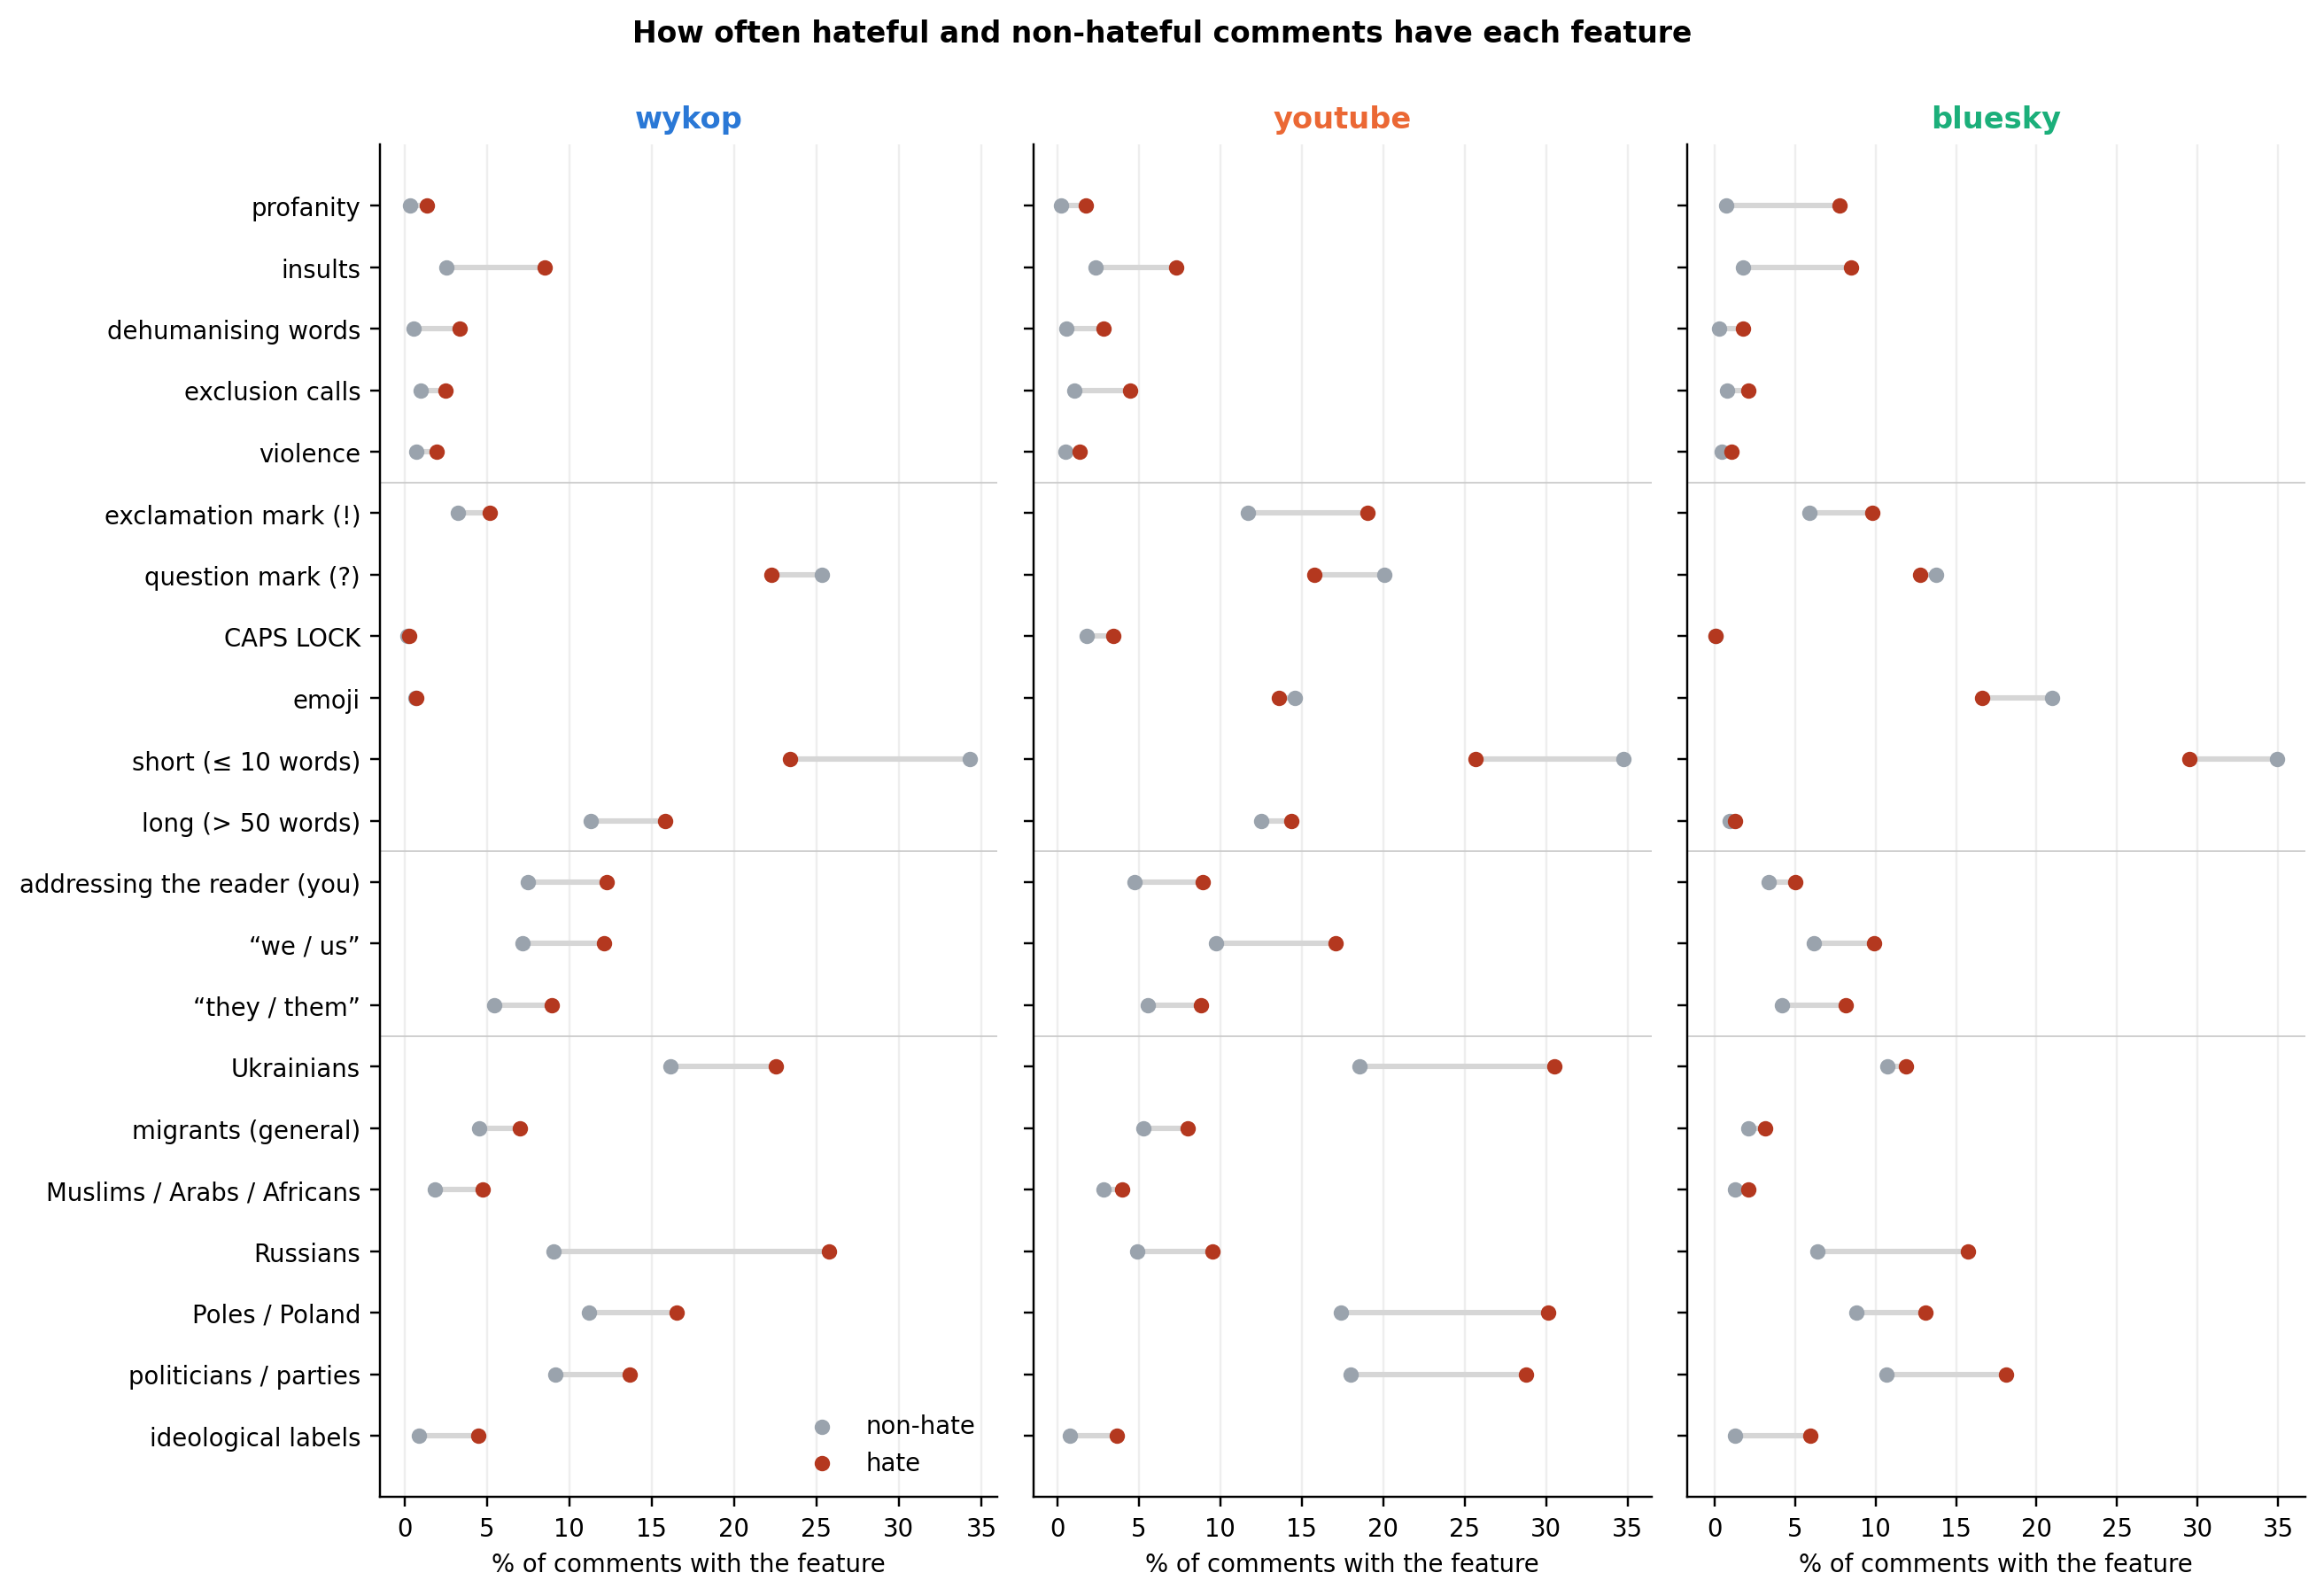
\includegraphics[width=0.9\textwidth]{ha_2_profile.png}
  \caption{How often hateful (red) and non-hateful (grey) comments have each feature, per platform. Features are detected with keyword lists and simple rules (e.g.\ ``CAPS LOCK'': at least 8 letters, at least half of them capitals). On Wykop, emoji and capital letters are almost absent from the collected text.}
  \label{fig:profile}
\end{figure*}

\subsection{Q2: How do hateful comments differ from other comments?}
\label{sec:q2}

For this question we use all 250,596 topic-filtered comments labelled by HerBERT in the 11 events. Figure~\ref{fig:profile} shows how often hateful and non-hateful comments have each feature, and Figure~\ref{fig:logit} shows which features are associated with hate when all of them are considered together.


\begin{figure}[tbp]
  \centering
  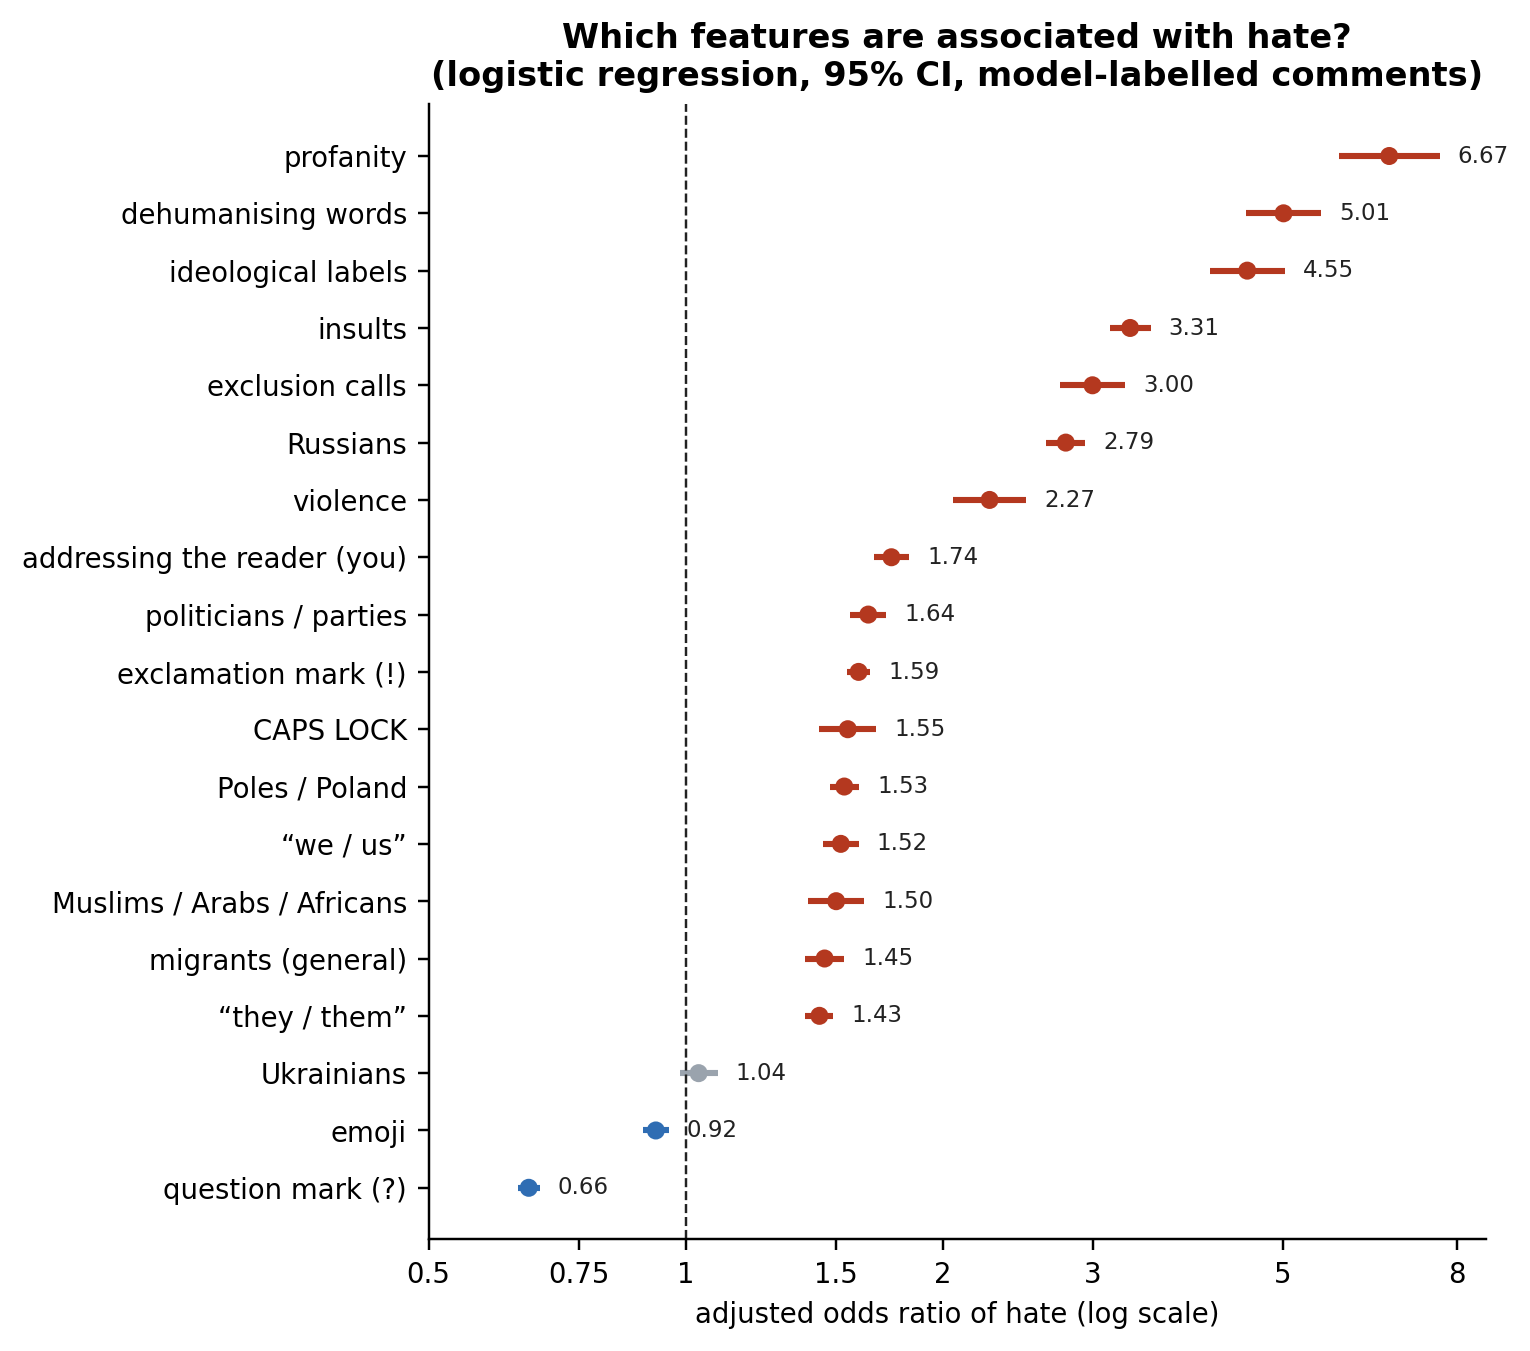
\includegraphics[width=\columnwidth]{ha_4_logit.png}
  \caption{Odds ratios from a logistic regression of hate on all features, log length and a separate baseline per cell (95\% CI clustered by thread; comments labelled by the slur dictionary excluded). Red: more likely hate; blue: less likely; grey: no association.}
  \label{fig:logit}
\end{figure}

\howtoread{An OR of 3 in Figure~\ref{fig:logit} means that a comment with this feature has three times higher odds of being hateful than an otherwise identical comment without it.}

\paragraph{Language, not topic.} The features most strongly associated with hate are profanity (OR 6.7), dehumanising words such as ``vermin'' or ``parasites'' (5.0), ideological labels such as \textit{lewak} `leftie', \textit{katol} or \textit{faszysta} (4.5), insults (3.3) and calls for exclusion such as ``get out'' or ``deport'' (3.0). In contrast, mentioning Ukrainians is not associated with hate once slur-based labels are excluded (OR 1.04, not significant). What makes a comment hateful is \emph{how} it speaks, not \emph{whom} it mentions.

\paragraph{Emotion and form.} Hateful comments more often contain exclamation marks (OR 1.6) and capital letters (1.5), and less often ask questions (0.66). They are slightly longer (median 20 vs.\ 15 words on Wykop, 19 vs.\ 15 on YouTube, 17 vs.\ 16 on Bluesky), but length itself is not associated with hate once the other features are taken into account: longer comments simply contain more insults and more mentions of groups.

\paragraph{``We'', ``they'' and ``you''.} Hate more often uses ``we/us'' (OR 1.5), ``they/such people'' (1.4) and refers to Poles (1.5). It also more often addresses the reader directly (``you'', 1.7): part of hate is aimed at other participants of the discussion, not at a group.

\paragraph{Not only migrants.} Mentions of Russians (OR 2.8) and of politicians and parties (1.6) are more strongly associated with hate than mentions of migrants (1.5). In discussions about migration, much of the general hate is political or anti-Russian. This is why we need a separate label for hate toward migrants.

\begin{figure}[tbp]
  \centering
  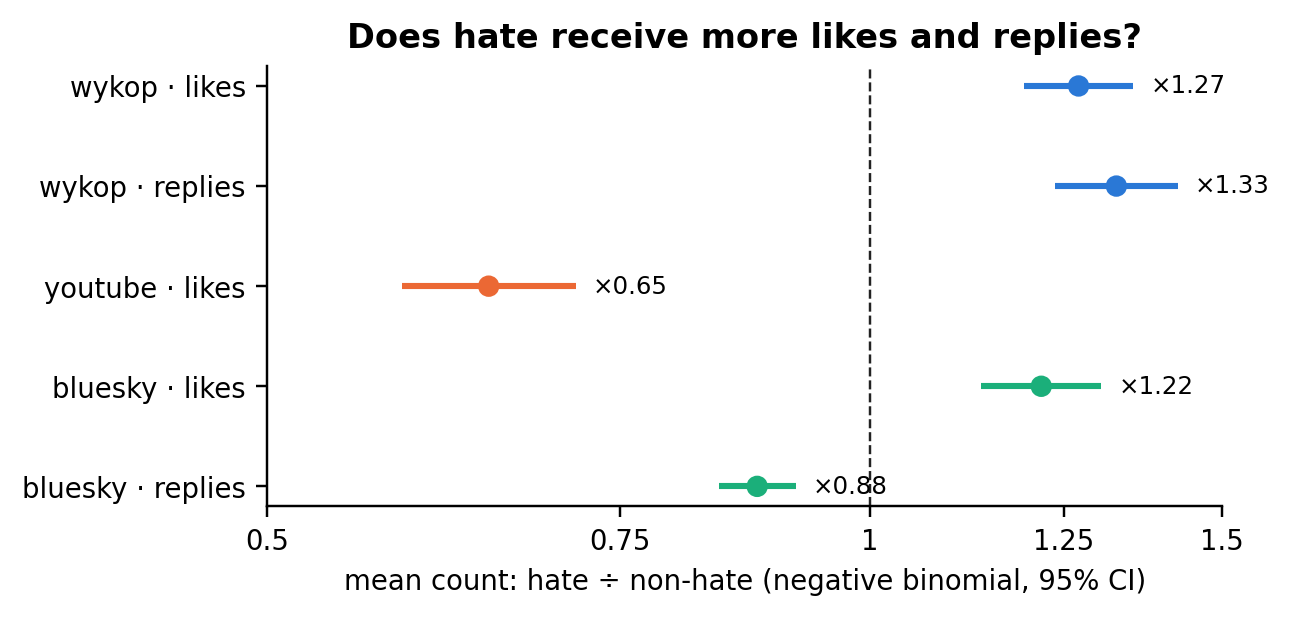
\includegraphics[width=0.95\columnwidth]{ha_5_engagement.png}
  \caption{Mean number of likes and replies of hateful comments divided by that of non-hateful comments (negative binomial model with a separate baseline per cell, 95\% CI). YouTube data contain no reply counts.}
  \label{fig:engagement}
\end{figure}

\paragraph{Engagement.} The reaction to hate depends on the platform (Figure~\ref{fig:engagement}). On Wykop, hateful comments receive more likes ($\times$1.27) and more replies ($\times$1.33) than other comments; on Bluesky they receive more likes ($\times$1.22) but fewer replies ($\times$0.88); on YouTube they receive clearly fewer likes ($\times$0.65).

\begin{figure}[tbp]
  \centering
  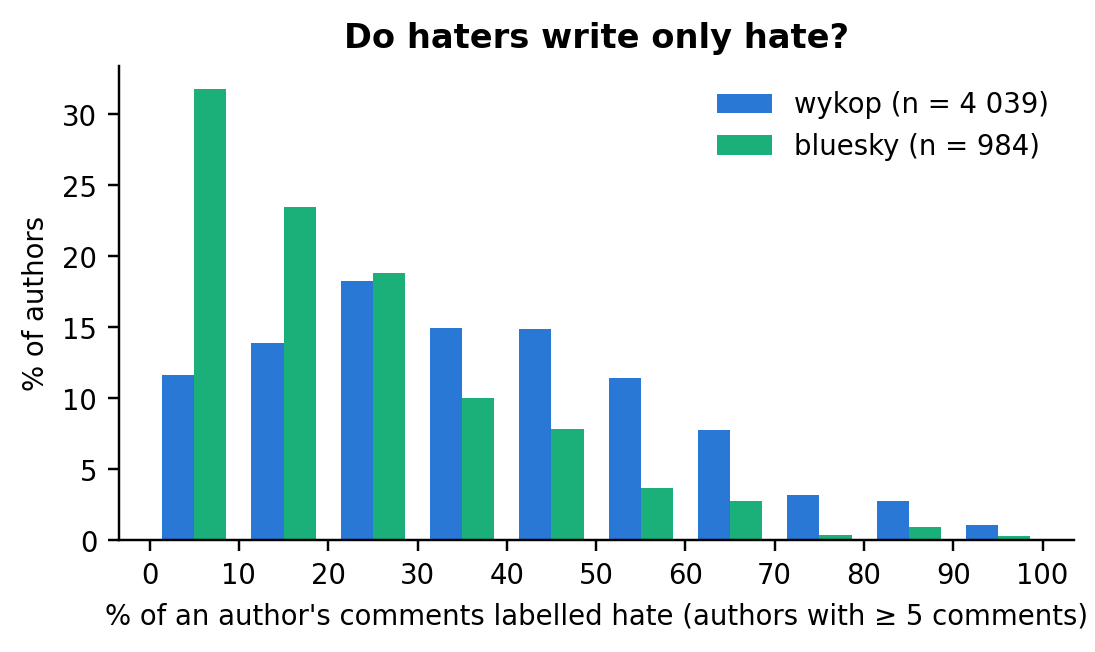
\includegraphics[width=0.95\columnwidth]{ha_6_authors.png}
  \caption{Share of hateful comments among all comments of an author, for authors with at least 5 comments.}
  \label{fig:haters}
\end{figure}

\paragraph{Do haters write only hate?} No (Figure~\ref{fig:haters}). At least one hateful comment was written by 58\% of authors on Wykop and 45\% on Bluesky. The 1\% most active haters wrote only 12--14\% of all hate. A typical active author mixes hateful and ordinary comments (median share of hate 33\% on Wykop and 17\% on Bluesky); only 2.5\% (Wykop) and 0.7\% (Bluesky) of active authors write almost only hate (more than 80\% of their comments).

% =====================================================================
\section{Discussion and Limitations}

Across three platforms and two independent labelling methods, salient events do not systematically increase hate speech toward migrants. Single events -- above all the adoption of the EU Pact -- produce clear and often short-lived increases, but others produce decreases, and on average the effect is zero. When hate increases, it is because migration becomes a topic of discussion: the share of hateful comments \emph{among} comments about migration stays the same. For monitoring, this means that the number of hateful comments after an event mostly measures attention, and that the share of hate within the topic is a more informative indicator. The platforms differ in their baseline level of hostility -- YouTube the most, Bluesky the least -- more than in how they react.

\paragraph{Limitations.}
(1) \textbf{Measurement.} The LLM misses about half of hateful comments, so the level of hate toward migrants is underestimated; our conclusions rely on changes within cells and agree across both pipelines. The gold standard was coded by two LLMs, with all disagreements resolved by a human; it is not a fully human-coded reference, and the pilot rounds show that even human coders often disagree.
(2) \textbf{Selection.} Only comments that pass the topic filter are labelled, so hate without migration-related words can be missed (equally before and after an event). Data collection differs between platforms, so levels are not comparable across them.
(3) \textbf{Number of events.} Seven (LLM) or eleven (HerBERT) events, with only one event of some types, make H2 exploratory. Bluesky has few comments for older events.
(4) \textbf{Causality.} A before--after comparison shows a change in time, not a causal effect; other news in the same period may contribute.
(5) \textbf{Features.} The features in Q2 are simple keyword rules and describe what HerBERT considers hateful.

% =====================================================================
\section{Conclusions}

Events related to migration change \emph{how much} users of Polish social media write about migrants more than \emph{how hostile} they are toward them. Some events, such as the adoption of the EU Pact, lead to clear increases in hate, but there is no general effect, the type of event does not explain the size of the reaction, and the three platforms react in similar ways despite very different levels of hate. Hate toward migrants is dominated by anti-Ukrainian vocabulary and shifts toward the group that an event is about. Hateful comments in general are marked by profanity, dehumanising words and ideological labels rather than by mentions of a particular group, and they are written by many users who mostly also write ordinary comments.


\bibliography{references}

\end{document}